\documentclass[%
  a4paper,%                                        % DIN A4
  oneside,%                                        % einseitiger Druck
  12pt,%                                           % 12pt Schriftgröße
]{article}

\usepackage[utf8]{inputenc}

% include required packages
\usepackage{url}
\usepackage{array}
\usepackage{color}
\usepackage{listings}
\usepackage{xspace}
\usepackage{tabularx}
\usepackage{hyperref}
%\usepackage{fancyhdr}
\usepackage{multicol}
\usepackage{capt-of}
\usepackage{graphicx}
\usepackage{float}

% HTML compilation
\usepackage{hevea}

% font setup
\usepackage{cmbright}
\usepackage{txfonts}
\usepackage[scaled=.90]{helvet}
\usepackage{courier}

% par. settings
\parindent 0pt
\parskip 8pt

\pretolerance=150
\tolerance=500
\hbadness=752

\pagenumbering{arabic}

\definecolor{lightgrey}{rgb}{0.9,0.9,0.9}
\definecolor{lightblue}{rgb}{0,0,1}

\definecolor{grey}{rgb}{0.5,0.5,0.5}
\definecolor{blue}{rgb}{0,0,1}
\definecolor{violet}{rgb}{0.5,0,0.5}

\definecolor{darkred}{rgb}{0.5,0,0}
\definecolor{darkblue}{rgb}{0,0,0.5}
\definecolor{darkgreen}{rgb}{0,0.5,0}


\newcommand{\sref}[1]{\S\,\ref{#1}}
\newcommand{\see}[1]{(see~\sref{#1})}

\newcommand{\singlefig}[3]{
  \begin{figure}[H]
    \centering
    \includegraphics[width=.6\columnwidth]{#1}
    \caption{#2}
    \label{#3}
  \end{figure}
}

\newcommand{\experimental}{
  {\color{darkred}\textsuperscript{experimental}}
}

\input{variables}

\title{%
%BEGIN LATEX
\libtitle
%END LATEX
\libsubtitle}

\author{Dominik Charousset}

\date{\today}

% page setup
\setlength{\voffset}{-1in}
\setlength{\hoffset}{-0.75in}
\addtolength{\textwidth}{1.5in}
\addtolength{\textheight}{2in}
\setlength{\headheight}{15pt}

% include paragraphs in TOC
\setcounter{tocdepth}{3}

% some HEVEA / HTML style sheets
\newstyle{body}{width:800px;margin:auto;padding-top:20px;text-align: justify;}
\newstyle{hr}{margin-top:10px;border-style:none;}

% more compact itemize
\newenvironment{itemize*}%
  {\begin{itemize}%
    \setlength{\itemsep}{0pt}%
    \setlength{\parskip}{0pt}}%
  {\end{itemize}}

\begin{document}
\maketitle\thispagestyle{empty}
\pagestyle{empty}
\clearpage
\tableofcontents
\clearpage
\setcounter{page}{1}
\pagestyle{plain}

% new highlight for INI file syntax
\begin{latexonly}
\lstdefinelanguage{ini}{%
  basicstyle=\ttfamily\footnotesize,%
%  columns=fullflexible,%
  morecomment=[s][\color{blue}]{[}{]},%
  morecomment=[l]{;},%
  morecomment=[s]{<}{>},%
  morestring=[b]",%
  morestring=[b]',%
  commentstyle=\color{violet},%
  morekeywords={},%
  otherkeywords={=,false,true},%
  keywordstyle=\color{blue},%
  stringstyle=\color{darkgreen},%
}
\end{latexonly}

% code listings setup
\lstset{%
  language=C++,%
  morekeywords={constexpr,nullptr,size_t,uint32_t,assert,override,final},%
  basicstyle=\ttfamily\footnotesize,%
  sensitive=true,%
  keywordstyle=\color{blue},%
  stringstyle=\color{darkgreen},%
  commentstyle=\color{violet},%
  showstringspaces=false,%
  tabsize=2,%
  frame=leftline,
  rulecolor=\color{lightblue},
  xleftmargin=20pt,
}

%BEGIN LATEX
\lstset{
  numberstyle=\tiny,
  numbers=left,
  numbersep=10pt,
  xleftmargin=20pt,
  %framesep=4.5mm,
  %framexleftmargin=2.5mm,
  framexleftmargin=5pt,
  framesep=15pt,
  fillcolor=\color{lightgrey},
}
%END LATEX

% content
\part{Core Library}
\section{Introduction}

Before diving into the API of \lib, we discuss the concepts behind it and explain the terminology used in this manual.

\subsection{Actor Model}

The actor model describes concurrent entities---actors---that do not share state and communicate only via asynchronous message passing.
Decoupling concurrently running software components via message passing avoids race conditions by design.
Actors can create---spawn---new actors and monitor each other to build fault-tolerant, hierarchical systems.
Since message passing is network transparent, the actor model applies to both concurrency and distribution.

Implementing applications on top of low-level primitives such as mutexes and semaphores has proven challenging and error-prone.
In particular when trying to implement applications that scale up to many CPU cores.
Queueing, starvation, priority inversion, and false sharing are only a few of the issues that can decrease performance significantly in mutex-based concurrency models.
In the extreme, an application written with the standard toolkit can run slower when adding more cores.

The actor model has gained momentum over the last decade due to its high level of abstraction and its ability to scale dynamically from one core to many cores and from one node to many nodes.
However, the actor model has not yet been widely adopted in the native programming domain.
With \lib, we contribute a library for actor programming in C++ as open-source software to ease native development of concurrent as well as distributed systems.
In this regard, \lib follows the C++ philosophy ``building the highest abstraction possible without sacrificing performance''.

\subsection{Terminology}

\lib is inspired by other implementations based on the actor model such as Erlang or Akka. It aims to provide a modern C++ API allowing for type-safe as well as dynamically typed messaging.
While there are similarities to other implementations, we made many different design decisions that lead to slight differences when comparing \lib to other actor frameworks.

\subsubsection{Dynamically Typed Actor}

A dynamically typed actor accepts any kind of message and dispatches on its content dynamically at the receiver.
This is the ``traditional'' messaging style found in implementations like Erlang or Akka.
The upside of this approach is (usually) faster prototyping and less code.
This comes at the cost of requiring excessive testing.

\subsubsection{Statically Typed Actor}

\lib achieves static type-checking for actors by defining abstract messaging interfaces.
Since interfaces define both input and output types, CAF is able to verify messaging protocols statically.
The upside of this approach is much higher robustness to code changes and fewer possible runtime errors.
This comes at an increase in required source code, as developers have to define and use messaging interfaces.

\subsubsection{Actor References}
\label{actor-reference}

\lib uses reference counting for actors. The three ways to store a reference to an actor are addresses, handles, and pointers. Note that \emph{address} does not refer to a \emph{memory region} in this context.

\paragraph{Address}
\label{actor-address}

Each actor has a (network-wide) unique logical address. This identifier is represented by \lstinline^actor_addr^, which allows to identify and monitor an actor.
Unlike other actor frameworks, \lib does \emph{not} allow users to send messages to addresses.
This limitation is due to the fact that the address does not contain any type information.
Hence, it would not be safe to send it a message, because the receiving actor might use a statically typed interface that does not accept the given message. Because an \lstinline^actor_addr^ fills the role of an identifier, it has \emph{weak reference semantics} \see{reference-counting}.

\paragraph{Handle}
\label{actor-handle}

An actor handle contains the address of an actor along with its type information and is required for sending messages to actors. The distinction between handles and addresses---which is unique to \lib when comparing it to other actor systems---is a consequence of the design decision to enforce static type checking for all messages. Dynamically typed actors use \lstinline^actor^ handles, while statically typed actors use \lstinline^typed_actor<...>^ handles. Both types have \emph{strong reference semantics} \see{reference-counting}.

\paragraph{Pointer}
\label{actor-pointer}

In a few instances, \lib uses \lstinline^strong_actor_ptr^ to refer to an actor using \emph{strong reference semantics} \see{reference-counting} without knowing the proper handle type. Pointers must be converted to a handle via \lstinline^actor_cast^ \see{actor-cast} prior to sending messages. A \lstinline^strong_actor_ptr^ can be \emph{null}.

\subsubsection{Spawning}

``Spawning'' an actor means to create and run a new actor.

\subsubsection{Monitor}
\label{monitor}

A monitored actor sends a down message~\see{down-message} to all actors monitoring it as part of its termination.
This allows actors to supervise other actors and to take actions when one of the supervised actors fails, i.e., terminates with a non-normal exit reason.

\subsubsection{Link}
\label{link}

A link is a bidirectional connection between two actors.
Each actor sends an exit message~\see{exit-message} to all of its links as part of its termination.
Unlike down messages, exit messages cause the receiving actor to terminate as well when receiving a non-normal exit reason per default.
This allows developers to create a set of actors with the guarantee that either all or no actors are alive.
Actors can override the default handler to implement error recovery strategies.

\subsection{Experimental Features}

Sections that discuss experimental features are highlighted with \experimental. The API of such features is not stable. This means even minor updates to \lib can come with breaking changes to the API or even remove a feature completely. However, we encourage developers to extensively test such features and to start discussions to uncover flaws, report bugs, or tweaking the API in order to improve a feature or streamline it to cover certain use cases.

\section{Overview}

Compiling \lib requires CMake and a C++11-compatible compiler. To get and compile the sources on UNIX-like systems, type the following in a terminal:

\begin{verbatim}
git clone https://github.com/actor-framework/actor-framework
cd actor-framework
./configure
make
make install [as root, optional]
\end{verbatim}

We recommended to run the unit tests as well:

\begin{verbatim}
make test
\end{verbatim}

If the output indicates an error, please submit a bug report that includes (a) your compiler version, (b) your OS, and (c) the content of the file \texttt{build/Testing/Temporary/LastTest.log}.

\subsection{Features}

\begin{itemize*}
  \item Lightweight, fast and efficient actor implementations
  \item Network transparent messaging
  \item Error handling based on Erlang's failure model
  \item Pattern matching for messages as internal DSL to ease development
  \item Thread-mapped actors for soft migration of existing applications
  \item Publish/subscribe group communication
\end{itemize*}


\subsection{Supported Compilers}

\begin{itemize*}
  \item GCC $\ge$ 4.8
  \item Clang $\ge$ 3.4
  \item Visual Studio $\ge$ 2015 (update 2)
\end{itemize*}

\subsection{Supported Operating Systems}

\begin{itemize*}
\item Linux
\item Mac OS X
\item Windows (static library only)
\end{itemize*}

\clearpage
\subsection{Hello World Example}

\lstinputlisting{../examples/hello_world.cpp}

\section{Message Handlers}
\label{message-handler}

Actors can store a set of callbacks---usually implemented as lambda expressions---using either \lstinline^behavior^ or \lstinline^message_handler^.
The former stores an optional timeout, while the latter is composable.

\subsection{Definition and Composition}

As the name implies, a \lstinline^behavior^ defines the response of an actor to messages it receives. The optional timeout allows an actor to dynamically change its behavior when not receiving message after a certain amount of time.

\begin{lstlisting}
message_handler x1{
  [](int i) { /*...*/ },
  [](double db) { /*...*/ },
  [](int a, int b, int c) { /*...*/ }
};
\end{lstlisting}

In our first example, \lstinline^x1^ models a behavior accepting messages that consist of either exactly one \lstinline^int^, or one \lstinline^double^, or three \lstinline^int^ values.
Any other message is not matched and gets forwarded to the default handler \see{default-handler}.

\begin{lstlisting}
message_handler x2{
  [](double db) { /*...*/ },
  [](double db) { /* - unrachable - */ }
};
\end{lstlisting}

Our second example illustrates an important characteristic of the matching mechanism. Each message is matched against the callbacks in the order they are defined. The algorithm stops at the first match. Hence, the second callback in \lstinline^x2^ is unreachable.

\begin{lstlisting}
message_handler x3 = x1.or_else(x2);
message_handler x4 = x2.or_else(x1);
\end{lstlisting}

Message handlers can be combined using \lstinline^or_else^. This composition is not commutative, as our third examples illustrates. The resulting message handler will first try to handle a message using the left-hand operand and will fall back to the right-hand operand if the former did not match. Thus, \lstinline^x3^ behaves exactly like \lstinline^x1^. This is because the second callback in \lstinline^x1^ will consume any message with a single \lstinline^double^ and both callbacks in \lstinline^x2^ are thus unreachable. The handler \lstinline^x4^ will consume messages with a single \lstinline^double^ using the first callback in \lstinline^x2^, essentially overriding the second callback in \lstinline^x1^.


\clearpage
\subsection{Atoms}
\label{atom}

Defining message handlers in terms of callbacks is convenient, but requires a simple way to annotate messages with meta data.
Imagine an actor that provides a mathematical service for integers.
It receives two integers, performs a user-defined operation and returns the result.
Without additional context, the actor cannot decide whether it should multiply or add the integers.
Thus, the operation must be encoded into the message.
The Erlang programming language introduced an approach to use non-numerical
constants, so-called \textit{atoms}, which have an unambiguous, special-purpose type and do not have the runtime overhead of string constants.

Atoms in \lib are mapped to integer values at compile time.
This mapping is guaranteed to be collision-free and invertible, but limits atom literals to ten characters and prohibits special characters.
Legal characters are \lstinline^_0-9A-Za-z^ and the whitespace character.
Atoms are created using the \lstinline^constexpr^ function \lstinline^atom^, as the following example illustrates.

\begin{lstlisting}
atom_value a1 = atom("add");
atom_value a2 = atom("multiply");
\end{lstlisting}

\textbf{Warning}: The compiler cannot enforce the restrictions at compile time, except for a length check.
The assertion \lstinline^atom("!?") != atom("?!")^ is not true, because each invalid character translates to a whitespace character.

While the \lstinline^atom_value^ is computed at compile time, it is not uniquely typed and thus cannot be used in the signature of a callback.
To accomplish this, \lib offers compile-time \emph{atom constants}.

\begin{lstlisting}
using add_atom = atom_constant<atom("add")>;
using multiply_atom = atom_constant<atom("multiply")>;
\end{lstlisting}

Using these constants, we can now define message passing interfaces in a convenient way:

\begin{lstlisting}
behavior do_math{
  [](add_atom, int a, int b) {
    return a + b;
  },
  [](multiply_atom, int a, int b) {
    return a * b;
  }
};

// caller side: send(math_actor, add_atom::value, 1, 2)
\end{lstlisting}

Atom constants define a static member \lstinline^value^.
Please note that this static \lstinline^value^ member does \emph{not} have the type \lstinline^atom_value^, unlike \lstinline^std::integral_constant^ for example.

\section{Actors}
\label{actor}

Actors in \lib are a lightweight abstraction for units of computations. They are active objects in the sense that they own their state and do not allow others to access it. The only way to modify the state of an actor is sending messages to it.

\lib provides several actor implementations, each covering a particular use case.
The available implementations differ in three characteristics: (1) dynamically or statically typed, (2) class-based or function-based, and (3) using asynchronous event handlers or blocking receives.
These three characteristics can be combined freely, with one exception: statically typed actors are always event-based.
For example, an actor can have dynamically typed messaging, implement a class, and use blocking receives.
The common base class for all user-defined actors is called \lstinline^local_actor^.

Dynamically typed actors are more familiar to developers coming from Erlang or Akka.
They (usually) enable faster prototyping but require extensive unit testing.
Statically typed actors require more source code but enable the compiler to verify communication between actors.
Since CAF supports both, developers can freely mix both kinds of actors to get the best of both worlds.
A good rule of thumb is to make use of static type checking for actors that are visible across multiple translation units.

Actors that utilize the blocking receive API always require an exclusive thread of execution. Event-based actors, on the other hand, are usually scheduled cooperatively and are very lightweight with a memory footprint of only few hundred bytes. Developers can exclude---detach---event-based actors that potentially starve others from the cooperative scheduling while spawning it. A detached actor lives in its own thread of execution.

\subsection{Environment / Actor Systems}
\label{actor-system}

All actors live in an \lstinline^actor_system^ representing an actor environment including scheduler~\see{scheduler}, registry~\see{registry}, and optional components such as a middleman~\see{middleman}. A single process can have multiple \lstinline^actor_system^ instances, but this is usually not recommended (a use case for multiple systems is to strictly separate two or more sets of actors by running them in different schedulers). For configuration and fine-tuning options of actor systems see \sref{system-config}. A distributed CAF application consists of two or more connected actor systems. We also refer to interconnected \lstinline^actor_system^ instances as a \emph{distributed actor system}.

\clearpage
\subsection{Common Actor Base Types}

The following pseudo-UML depicts the class diagram for actors in \lib. Irrelevant member functions and classes as well as mixins are omitted for brevity. Selected individual classes are presented in more detail in the following sections.

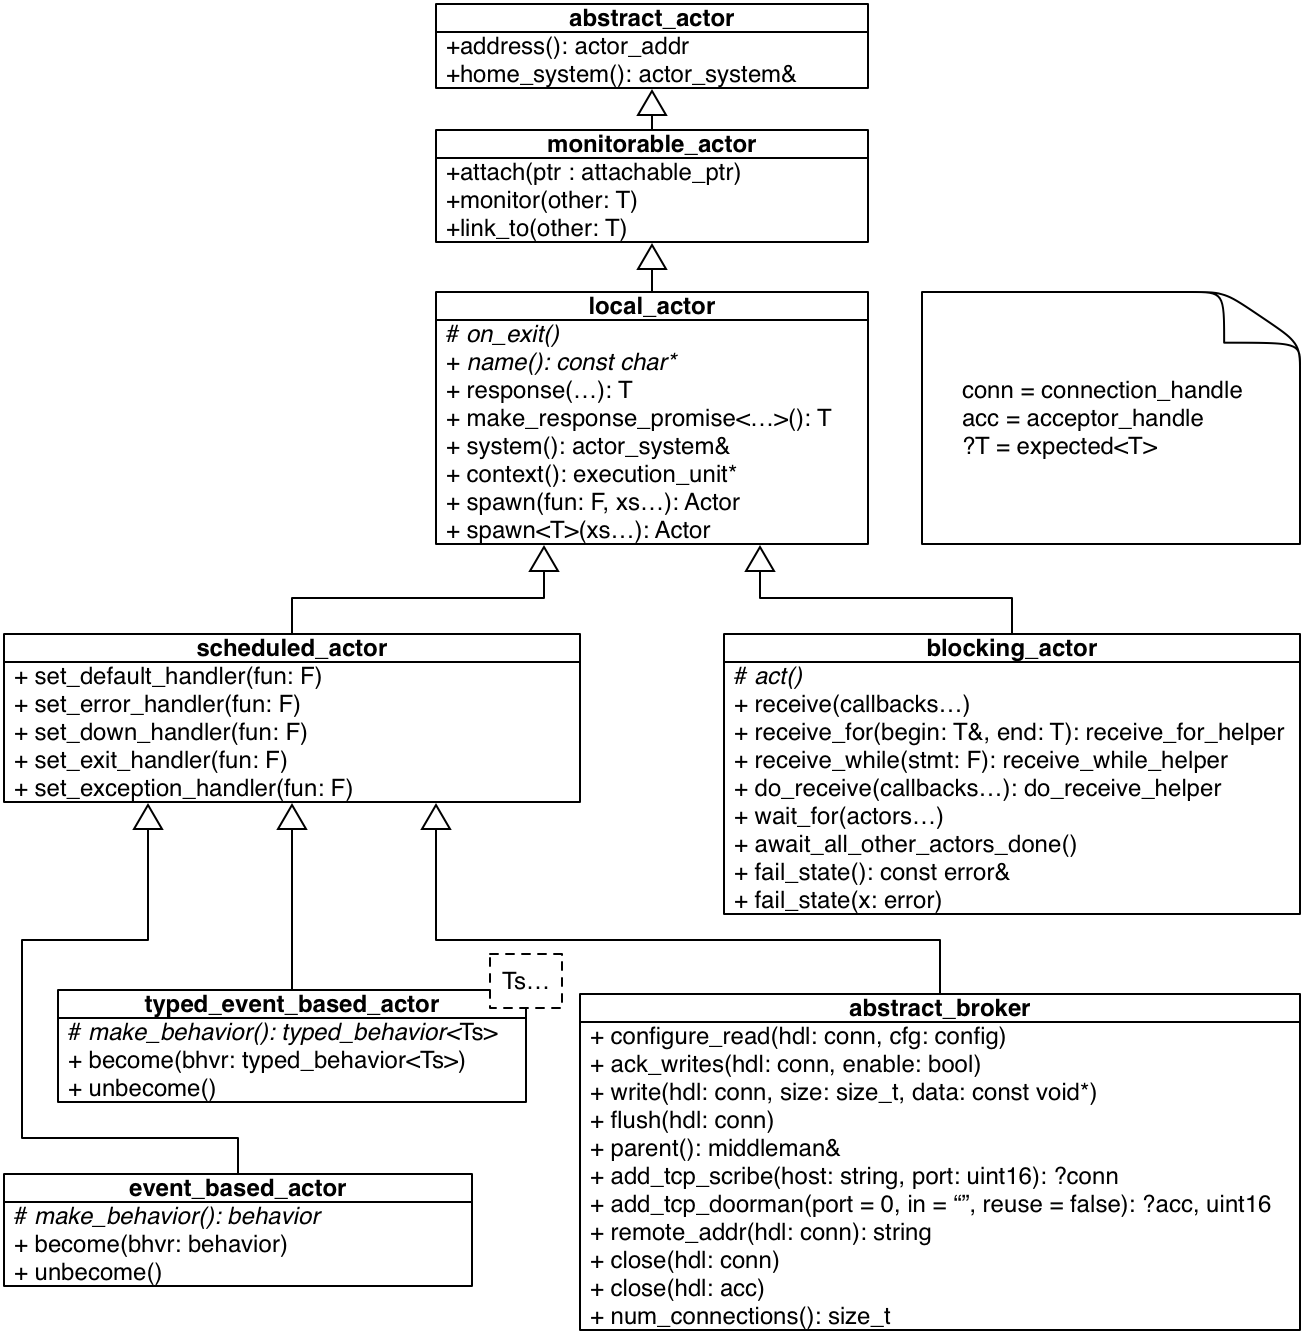
\includegraphics[width=\textwidth]{actor_types}

\clearpage
\subsubsection{Class \lstinline^local_actor^}

The class \lstinline^local_actor^ is the root type for all user-defined actors in \lib. It defines all common operations.
However, users of the library usually do not inherit from this class directly. Proper base classes for user-defined actors are \lstinline^event_based_actor^ or \lstinline^blocking_actor^. The following table also includes member function inherited from \lstinline^monitorable_actor^ and \lstinline^abstract_actor^.

\begin{center}
\small
\begin{tabular}{ll}
  \textbf{Types} & ~ \\
  \hline
  \lstinline^mailbox_type^ & A concurrent, many-writers-single-reader queue type. \\
  \hline
  ~ & ~ \\ \textbf{Constructors} & ~ \\
  \hline
  \lstinline^(actor_config&)^ & Constructs the actor using a config. \\
  \hline
  ~ & ~ \\ \textbf{Observers} & ~ \\
  \hline
  \lstinline^actor_addr address()^ & Returns the address of this actor. \\
  \hline
  \lstinline^actor_system& system()^ & Returns \lstinline^context()->system()^. \\
  \hline
  \lstinline^actor_system& home_system()^ & Returns the system that spawned this actor. \\
  \hline
  \lstinline^execution_unit* context()^ & Returns underlying thread or current scheduler worker. \\
  \hline
  ~ & ~ \\ \textbf{Customization Points} & ~ \\
  \hline
  \lstinline^on_exit()^ & Can be overridden to perform cleanup code. \\
  \hline
  \lstinline^const char* name()^ & Returns a debug name for this actor type. \\
  \hline
  ~ & ~ \\ \textbf{Actor Management} & ~ \\
  \hline
  \lstinline^link_to(other)^ & Link to an actor \see{link}. \\
  \hline
  \lstinline^unlink_from(other)^ & Remove link to an actor \see{link}. \\
  \hline
  \lstinline^monitor(other)^ & Unidirectionally monitors an actor \see{monitor}. \\
  \hline
  \lstinline^demonitor(other)^ & Removes a monitor from \lstinline^whom^. \\
  \hline
  \lstinline^spawn(F fun, xs...)^ & Spawns a new actor from \lstinline^fun^. \\
  \hline
  \lstinline^spawn<T>(xs...)^ & Spawns a new actor of type \lstinline^T^. \\
  \hline
  ~ & ~ \\ \textbf{Message Processing} & ~ \\
  \hline
  \lstinline^T make_response_promise<Ts...>()^ & Allows an actor to delay its response message. \\
  \hline
  \lstinline^T response(xs...)^ & Convenience function for creating fulfilled promises. \\
  \hline
\end{tabular}
\end{center}

\clearpage
\subsubsection{Class \lstinline^scheduled_actor^}

All scheduled actors inherit from \lstinline^scheduled_actor^. This includes statically and dynamically typed event-based actors as well as brokers \see{broker}.

\begin{center}
\small
\begin{tabular}{ll}
  \textbf{Types} & ~ \\
  \hline
  \lstinline^pointer^ & \lstinline^scheduled_actor*^ \\
  \hline
  \lstinline^exception_handler^ & \lstinline^function<error (pointer, std::exception_ptr&)>^ \\
  \hline
  \lstinline^default_handler^ & \lstinline^function<result<message> (pointer, message_view&)>^ \\
  \hline
  \lstinline^error_handler^ & \lstinline^function<void (pointer, error&)>^ \\
  \hline
  \lstinline^down_handler^ & \lstinline^function<void (pointer, down_msg&)>^ \\
  \hline
  \lstinline^exit_handler^ & \lstinline^function<void (pointer, exit_msg&)>^ \\
  \hline
  ~ & ~ \\ \textbf{Constructors} & ~ \\
  \hline
  \lstinline^(actor_config&)^ & Constructs the actor using a config. \\
  \hline
  ~ & ~ \\ \textbf{Termination} & ~ \\
  \hline
  \lstinline^quit()^ & Finishes execution of this actor without error (``normal exit reason''). \\
  \hline
  \lstinline^quit(error x)^ & Finishes execution of this actor with error \lstinline^x^. \\
  \hline
  ~ & ~ \\ \textbf{Special-purpose Handlers} & ~ \\
  \hline
  \lstinline^set_exception_handler(F f)^ & Installs \lstinline^f^ for converting exceptions to errors \see{error}. \\
  \hline
  \lstinline^set_down_handler(F f)^ & Installs \lstinline^f^ to handle down messages \see{down-message}. \\
  \hline
  \lstinline^set_exit_handler(F f)^ & Installs \lstinline^f^ to handle exit messages \see{exit-message}. \\
  \hline
  \lstinline^set_error_handler(F f)^ & Installs \lstinline^f^ to handle error messages (see \sref{error-message} and \sref{error}). \\
  \hline
  \lstinline^set_default_handler(F f)^ & Installs \lstinline^f^ as fallback message handler \see{default-handler}. \\
  \hline
\end{tabular}
\end{center}

\clearpage
\subsubsection{Class \lstinline^blocking_actor^}

A blocking actor always lives in its own thread of execution. They are not as lightweight as event-based actors and thus do not scale up to large numbers. The primary use case for blocking actors is to use a \lstinline^scoped_actor^ for ad-hoc communication to selected actors. Unlike scheduled actors, \lib does \textbf{not} dispatch system messages to special-purpose handlers. A blocking actors receives \emph{all} messages regularly through its mailbox. A blocking actor is considered \emph{done} only after it returned from \lstinline^act^ (or from the implementation in function-based actors). A \lstinline^scoped_actor^ sends its exit messages as part of its destruction.

\begin{center}
\small
\begin{tabular}{ll}
  \textbf{Constructors} & ~ \\
  \hline
  \lstinline^(actor_config&)^ & Constructs the actor using a config. \\
  \hline
  ~ & ~ \\ \textbf{Customization Points} & ~ \\
  \hline
  \lstinline^void act()^ & Implements the behavior of the actor. \\
  \hline
  ~ & ~ \\ \textbf{Termination} & ~ \\
  \hline
  \lstinline^const error& fail_state()^ & Returns the current exit reason. \\
  \hline
  \lstinline^fail_state(error x)^ & Sends \lstinline^x^ to other actors as exit reason after this actor is done. \\
  \hline
  ~ & ~ \\ \textbf{Actor Management} & ~ \\
  \hline
  \lstinline^wait_for(Ts... xs)^ & Blocks until all actors \lstinline^xs...^ are done. \\
  \hline
  \lstinline^await_all_other_actors_done()^ & Blocks until all other actors are done. \\
  \hline
  ~ & ~ \\ \textbf{Message Handling} & ~ \\
  \hline
  \lstinline^receive(Ts... xs)^ & Receives a message using the callbacks \lstinline^xs...^. \\
  \hline
  \lstinline^receive_for(T& begin, T end)^ & See \sref{receive-loop}. \\
  \hline
  \lstinline^receive_while(F stmt)^ & See \sref{receive-loop}. \\
  \hline
  \lstinline^do_receive(Ts... xs)^ & See \sref{receive-loop}. \\
  \hline
\end{tabular}
\end{center}

\clearpage
\subsection{Messaging Interfaces}
\label{interface}

Statically typed actors require abstract messaging interfaces to allow the compiler to type-check actor communication.
Interfaces in CAF are defined using the variadic template \lstinline^typed_actor<...>^, which defines the proper actor handle at the same time.
Each template parameter defines one \lstinline^input -> output^ pair via \lstinline^replies_to<X1,...,Xn>::with<Y1,...,Yn>^.
For inputs that do not generate outputs, \lstinline^reacts_to<X1,...,Xn>^ can be used as shortcut for \lstinline^replies_to<X1,...,Xn>::with<void>^. In the same way functions cannot be overloaded only by their return type, interfaces cannot accept one input twice (possibly mapping it to different outputs). The example below defines a messaging interface for a simple calculator.

\lstinputlisting[linerange={17-21}]{../examples/message_passing/calculator.cpp}

It is not required to create a type alias such as \lstinline^calculator_actor^, but it makes dealing with statically typed actors much easier.
Also, a central alias definition eases refactoring later on.

Interfaces have set semantics. This means the following two type aliases \lstinline^i1^ and \lstinline^i2^ are equal:

\begin{lstlisting}
using i1 = typed_actor<replies_to<A>::with<B>, replies_to<C>::with<D>>;
using i2 = typed_actor<replies_to<C>::with<D>, replies_to<A>::with<B>>;
\end{lstlisting}

Further, actor handles of type \lstinline^A^ are assignable to handles of type \lstinline^B^ as long as \lstinline^B^ is a subset of \lstinline^A^.

For convenience, the class \lstinline^typed_actor<...>^ defines the member types shown below to grant access to derived types.

\begin{center}
\small
\begin{tabular}{ll}
  \textbf{Types} & ~ \\
  \hline
  \lstinline^behavior_type^ & A statically typed set of message handlers. \\
  \hline
  \lstinline^base^ & Base type for actors, i.e., \lstinline^typed_event_based_actor<...>^. \\
  \hline
  \lstinline^pointer^ & A pointer of type \lstinline^base*^. \\
  \hline
  \lstinline^stateful_base<T>^ & See \sref{stateful-actor}. \\
  \hline
  \lstinline^stateful_pointer<T>^ & A pointer of type \lstinline^stateful_base<T>*^. \\
  \hline
  \lstinline^extend<Ts...>^ & Extend this typed actor with \lstinline^Ts...^. \\
  \hline
  \lstinline^extend_with<Other>^ & Extend this typed actor with all cases from \lstinline^Other^. \\
  \hline
\end{tabular}
\end{center}

\clearpage
\subsection{Spawning Actors}
\label{spawn}

Both statically and dynamically typed actors are spawned from an \lstinline^actor_system^ using the member function \lstinline^spawn^. The function either takes a function as first argument or a class as first template parameter. For example, the following functions and classes represent actors.

\lstinputlisting[linerange={24-29}]{../examples/message_passing/calculator.cpp}

Spawning an actor for each implementation is illustrated below.

\lstinputlisting[linerange={140-145}]{../examples/message_passing/calculator.cpp}

Additional arguments to \lstinline^spawn^ are passed to the constructor of a class or used as additional function arguments, respectively. In the example above, none of the three functions takes any argument other than the implicit but optional \lstinline^self^ pointer.

\subsection{Function-based Actors}
\label{function-based}

When using a function or function object to implement an actor, the first argument \emph{can} be used to capture a pointer to the actor itself.
The type of this pointer is usually \lstinline^event_based_actor*^ or \lstinline^blocking_actor*^.
The proper pointer type for any \lstinline^typed_actor^ handle \lstinline^T^ can be obtained via \lstinline^T::pointer^ \see{interface}.

Blocking actors simply implement their behavior in the function body. The actor is done once it returns from that function.

Event-based actors can either return a \lstinline^behavior^ \see{message-handler} that is used to initialize the actor or explicitly set the initial behavior by calling \lstinline^self->become(...)^. Due to the asynchronous, event-based nature of this kind of actor, the function usually returns immediately after setting a behavior (message handler) for the \emph{next} incoming message. Hence, variables on the stack will be out of scope once a message arrives. Managing state in function-based actors can be done either via rebinding state with \lstinline^become^, using heap-located data referenced via \lstinline^std::shared_ptr^ or by using the ``stateful actor'' abstraction~\see{stateful-actor}.

The following three functions implement the prototypes shown in~\sref{spawn} and illustrate one blocking actor and two event-based actors (statically and dynamically typed).

\clearpage
\lstinputlisting[linerange={31-72}]{../examples/message_passing/calculator.cpp}

\clearpage
\subsection{Class-based Actors}
\label{class-based}

Implementing an actor using a class requires the following:
\begin{itemize}
\item Provide a constructor taking a reference of type \lstinline^actor_config&^ as first argument, which is forwarded to the base class. The config is passed implicitly to the constructor when calling \lstinline^spawn^, which also forwards any number of additional arguments to the constructor.
\item Override \lstinline^make_behavior^ for event-based actors and \lstinline^act^ for blocking actors.
\end{itemize}

Implementing actors with classes works for all kinds of actors and allows simple management of state via member variables. However, composing states via inheritance can get quite tedious. For dynamically typed actors, composing states is particularly hard, because the compiler cannot provide much help. For statically typed actors, \lib also provides an API for composable behaviors~\see{composable-behavior} that works well with inheritance. The following three examples implement the forward declarations shown in \sref{spawn}.

\lstinputlisting[linerange={74-108}]{../examples/message_passing/calculator.cpp}

\clearpage
\subsection{Stateful Actors}
\label{stateful-actor}

The stateful actor API makes it easy to maintain state in function-based actors. It is also safer than putting state in member variables, because the state ceases to exist after an actor is done and is not delayed until the destructor runs. For example, if two actors hold a reference to each other via member variables, they produce a cycle and neither will get destroyed. Using stateful actors instead breaks the cycle, because references are destroyed when an actor calls \lstinline^self->quit()^ (or is killed externally). The following example illustrates how to implement stateful actors with static typing as well as with dynamic typing.

\lstinputlisting[linerange={18-44}]{../examples/message_passing/cell.cpp}

Stateful actors are spawned in the same way as any other function-based actor \see{function-based}.

\lstinputlisting[linerange={49-50}]{../examples/message_passing/cell.cpp}

\clearpage
\subsection{Actors from Composable Behaviors \experimental}
\label{composable-behavior}

When building larger systems, it is often useful to implement the behavior of an actor in terms of other, existing behaviors. The composable behaviors in \lib allow developers to generate a behavior class from a messaging interface~\see{interface}.

The base type for composable behaviors is \lstinline^composable_behavior<T>^, where \lstinline^T^ is a \lstinline^typed_actor<...>^. \lib maps each \lstinline^replies_to<A, B, C>::with<D, E, F>^ in \lstinline^T^ to a pure virtual member function with signature \lstinline^result<D, E, F> operator()(param<A>, param<B>, param<C>)^.

Note that \lstinline^operator()^ will take integral types as well as atom constants simply by value. A \lstinline^result<T>^ accepts either a value of type \lstinline^T^, a \lstinline^skip_t^ \see{default-handler}, an \lstinline^error^ \see{error}, a \lstinline^delegated<T>^ \see{delegate}, or a \lstinline^response_promise<T>^ \see{promise}. A \lstinline^result<void>^ is constructed by returning \lstinline^unit^.

A behavior that combines the behaviors \lstinline^X^, \lstinline^Y^, and \lstinline^Z^ must inherit from \lstinline^composed_behavior<X, Y, Z>^ instead of inheriting from the three classes directly. The class \lstinline^composed_behavior^ ensures that the behaviors are concatenated correctly. In case one message handler is defined in multiple base types, the \emph{first} type in declaration order ``wins''. For example, if \lstinline^X^ and \lstinline^Y^ both implement the interface \lstinline^replies_to<int, int>::with<int>^, only the handler implemented in \lstinline^X^ is active.

Any composable (or composed) behavior with no pure virtual member functions can be spawned directly through an actor system by calling \lstinline^system.spawn<...>()^, as shown below.

\lstinputlisting[linerange={20-52}]{../examples/composition/calculator_behavior.cpp}

\clearpage
The second example illustrates how to use non-primitive values that are wrapped in a \lstinline^param<T>^ when working with composable behaviors. The purpose of \lstinline^param<T>^ is to provide a single interface for both constant and non-constant access. Constant access is modeled with the implicit conversion operator to \lstinline^const T&^, the member function \lstinline^get()^ and \lstinline^operator->^. 

When acquiring mutable access to the represented value, CAF copies the value before allowing mutable access to it if more than one reference to the value exists. This copy-on-write optimization avoids race conditions by design, while minimizing copy operations \see{copy-on-write}. A mutable reference is returned from the member functions \lstinline^get_mutable()^ and \lstinline^move()^. The latter is a convenience function for \lstinline^std::move(x.get_mutable())^. The following example illustrates how to use \lstinline^param<std::string>^ when implementing a simple dictionary.

\lstinputlisting[linerange={22-44}]{../examples/composition/dictionary_behavior.cpp}

\subsection{Attaching Cleanup Code to Actors}
\label{attach}

Users can attach cleanup code to actors. This code is executed immediately if the actor has already exited. Otherwise, the actor will execute it as part of its termination. The following example attaches a function object to actors for printing a custom string on exit.

\lstinputlisting[linerange={46-50}]{../examples/broker/simple_broker.cpp}

It is possible to attach code to remote actors. However, the cleanup code will run on the local machine.

\subsection{Blocking Actors}
\label{blocking-actor}

Blocking actors always run in a separate thread and are not scheduled by \lib. Unlike event-based actors, blocking actors have explicit, blocking \emph{receive} functions. Further, blocking actors do not handle system messages automatically via special-purpose callbacks \see{special-handler}. This gives users full control over the behavior of blocking actors. However, blocking actors still should follow conventions of the actor system. For example, actors should unconditionally terminate after receiving an \lstinline^exit_msg^ with reason \lstinline^exit_reason::kill^.

\subsubsection{Receiving Messages}

The function \lstinline^receive^ sequentially iterates over all elements in the mailbox beginning with the first.
It takes a message handler that is applied to the elements in the mailbox until an element was matched by the handler.
An actor calling \lstinline^receive^ is blocked until it successfully dequeued a message from its mailbox or an optional timeout occurs. Messages that are not matched by the behavior are automatically skipped and remain in the mailbox.

\begin{lstlisting}
self->receive (
  [](int x) { /* ... */ }
);
\end{lstlisting}

\subsubsection{Catch-all Receive Statements}
\label{catch-all}

Blocking actors can use inline catch-all callbacks instead of setting a default handler \see{default-handler}. A catch-all case must be the last callback before the optional timeout, must be prefixed with \lstinline^others >>^, and must have the signature \lstinline^result<message> (const type_erased_tuple*)^.

The following example showcases a simple receive statement that expects a \lstinline^float^ and handles the system messages \lstinline^down_msg^ and \lstinline^exit_msg^. If neither of these three cases match, the actor reports an error back to the sender.

\begin{lstlisting}
self->receive(
  [&](float x) {
    // ...
  },
  [&](const down_msg& x) {
    // ...
  },
  [&](const exit_msg& x) {
    // ...
  },
  others >> [](message_view& x) -> result<message> {
    // report unexpected message back to client
    return sec::unexpected_message;
  }
);
\end{lstlisting}

\clearpage
\subsubsection{Receive Loops}
\label{receive-loop}

Message handler passed to \lstinline^receive^ are temporary object at runtime.
Hence, calling \lstinline^receive^ inside a loop creates an unnecessary amount of short-lived objects.
\lib provides predefined receive loops to allow for more efficient code.

\begin{lstlisting}
// BAD
std::vector<int> results;
for (size_t i = 0; i < 10; ++i)
  receive (
    [&](int value) {
      results.push_back(value);
    }
  );

// GOOD
std::vector<int> results;
size_t i = 0;
receive_for(i, 10) (
  [&](int value) {
    results.push_back(value);
  }
);
\end{lstlisting}

\begin{lstlisting}
// BAD
size_t received = 0;
while (received < 10) {
  receive (
    [&](int) {
      ++received;
    }
  );
} ;

// GOOD
size_t received = 0;
receive_while([&] { return received < 10; }) (
  [&](int) {
    ++received;
  }
);
\end{lstlisting}
\clearpage

\begin{lstlisting}
// BAD
size_t received = 0;
do {
  receive (
    [&](int) {
      ++received;
    }
  );
} while (received < 10);

// GOOD
size_t received = 0;
do_receive (
  [&](int) {
    ++received;
  }
).until([&] { return received >= 10; });
\end{lstlisting}

The examples above illustrate the correct usage of the three loops \lstinline^receive_for^, \lstinline^receive_while^ and \lstinline^do_receive(...).until^.
It is possible to nest receives and receive loops.

\begin{lstlisting}
bool running = true;
self->receive_while([&] { return running; }) (
  [&](int value1) {
    self->receive (
      [&](float value2) {
        aout(self) << value1 << " => " << value2 << endl;
      }
    );
  },
  // ...
);
\end{lstlisting}

\subsubsection{Scoped Actors}
\label{scoped-actors}

The class \lstinline^scoped_actor^ offers a simple way of communicating with CAF actors from non-actor contexts.
It overloads \lstinline^operator->^ to return a \lstinline^blocking_actor*^.
Hence, it behaves like the implicit \lstinline^self^ pointer in functor-based actors, only that it ceases to exist at scope end.

\begin{lstlisting}
void test(actor_system& system) {
  scoped_actor self{system};
  // spawn some actor
  auto aut = self->spawn(my_actor_impl);
  self->send(aut, "hi there");
  // self will be destroyed automatically here; any
  // actor monitoring it will receive down messages etc.
}
\end{lstlisting}

\section{Message Passing}
\label{message-passing}

Message passing in CAF is always asynchronous. Further, CAF neither guarantees message delivery nor message ordering in a distributed setting. CAF uses TCP per default, but also enables nodes to send messages to other nodes without having a direct connection.  In this case, messages are forwarded by intermediate nodes and can get lost if one of the forwarding nodes fails. Likewise, forwarding paths can change dynamically and thus cause messages to arrive out of order.

The messaging layer of CAF has three primitives for sending messages: \lstinline^send^, \lstinline^request^, and \lstinline^delegate^. The former simply enqueues a message to the mailbox the receiver. The latter two are discussed in more detail in \sref{request} and \sref{delegate}.

\subsection{Structure of Mailbox Elements}
\label{mailbox-element}

When enqueuing a message to the mailbox of an actor, \lib wraps the content of the message into a \lstinline^mailbox_element^ (shown below) to add meta data and processing paths.

{\footnotesize
\begin{verbatim}
     +-----------------+
     | mailbox_element |
     +-----------------+
     | sender          |
     | message ID      |
     | stages          |
     | content         |
     +-----------------+
\end{verbatim}}

The sender is stored as a \lstinline^strong_actor_ptr^ \see{actor-pointer} and denotes the origin of the message. The message ID is either 0---invalid---or a positive integer value that allows the sender to match a response to its request. The \lstinline^stages^ vector stores the path of the message. Response messages, i.e., the returned values of a message handler, are sent to \lstinline^stages.back()^ after calling \lstinline^stages.pop_back()^. This allows \lib to build pipelines of arbitrary size. If no more stage is left, the response reaches the sender. Finally, \lstinline^content^ is a \lstinline^message^ object~\see{message} storing a type-erased tuple.

Mailbox elements are created by \lib automatically and are usually invisible to the programmer. However, understanding how messages are processed internally helps understanding the behavior of the message passing layer.

It is worth mentioning that \lib usually wraps the mailbox element and its content into a single object in order to reduce the number of memory allocations.

\subsection{Default and System Message Handlers}
\label{special-handler}

\lib has three system-level message types (\lstinline^down_msg^, \lstinline^exit_msg^, and \lstinline^error^) that all actor should handle regardless of there current state. Consequently, event-based actors handle such messages in special-purpose message handlers. Additionally, event-based actors have a fallback handler for unmatched messages. Note that blocking actors have neither of those special-purpose handlers \see{blocking-actor}.

\subsubsection{Down  Handler}
\label{down-message}

Actors can monitor the lifetime of other actors by calling \lstinline^self->monitor(other)^. This will cause the runtime system of \lib to send a \lstinline^down_msg^ for \lstinline^other^ if it dies. Actors drop down messages unless they provide a custom handler via \lstinline^set_down_handler(f)^, where \lstinline^f^ is a function object with signature \lstinline^void (down_message&)^ or \lstinline^void (scheduled_actor*, down_message&)^. The latter signature allows users to implement down message handlers as free function.

\subsubsection{Exit Handler}
\label{exit-message}

Bidirectional monitoring with a strong lifetime coupling is established by calling \lstinline^self->link_to(other)^. This will cause the runtime to send an \lstinline^exit_msg^ if either \lstinline^this^ or \lstinline^other^ dies. Per default, actors terminate after receiving an \lstinline^exit_msg^ unless the exit reason is \lstinline^exit_reason::normal^. This mechanism propagates failure states in an actor system. Linked actors form a sub system in which an error causes all actors to fail collectively. Actors can override the default handler via \lstinline^set_exit_handler(f)^, where \lstinline^f^ is a function object with signature \lstinline^void (exit_message&)^ or \lstinline^void (scheduled_actor*, exit_message&)^.

\subsubsection{Error Handler}
\label{error-message}

Actors send error messages to others by returning an \lstinline^error^ \see{error} from a message handler. Similar to exit messages, error messages usually cause the receiving actor to terminate, unless a custom handler was installed via \lstinline^set_error_handler(f)^, where \lstinline^f^ is a function object with signature \lstinline^void (error&)^ or \lstinline^void (scheduled_actor*, error&)^. Additionally, \lstinline^request^ accepts an error handler as second argument to handle errors for a particular request~\see{error-response}. The default handler is used as fallback if \lstinline^request^ is used without error handler. 

\subsubsection{Default Handler}
\label{default-handler}

The default handler is called whenever the behavior of an actor did not match the input. Actors can change the default handler by calling \lstinline^set_default_handler^. The expected signature of the function object is \lstinline^result<message> (scheduled_actor*, const type_erased_tuple*)^, whereas the \lstinline^self^ pointer can again be omitted. The default handler can return a response message or cause the runtime to \emph{skip} the input message to allow an actor to handle it in a later state. \lib provides the following built-in implementations: \lstinline^reflect^, \lstinline^reflect_and_quit^, \lstinline^print_and_drop^, \lstinline^drop^, and \lstinline^skip^. The former two are meant for debugging and testing purposes and allow an actor to simply return an input. The next two functions drop unexpected messages with or without printing a warning beforehand. Finally, \lstinline^skip^ leaves the input message in the mailbox. The default is \lstinline^print_and_drop^.

\subsection{Requests}
\label{request}

A main feature of \lib is its ability to couple input and output types via the type system. For example, a \lstinline^typed_actor<replies_to<int>::with<int>>^ essentially behaves like a function. It receives a single \lstinline^int^ as input and responds with another \lstinline^int^. \lib embraces this functional take on actors by simply creating response messages from the result of message handlers. This allows \lib to match \emph{request} to \emph{response} messages and to provide a convenient API for this style of communication.

\subsubsection{Sending Requests and Handling Responses}
\label{handling-response}

Actors send request messages by calling \lstinline^request(receiver, timeout, content...)^. This function returns an intermediate object that allows an actor to set a one-shot handler for the response message. Event-based actors can use either \lstinline^request(...).then^ or \lstinline^request(...).await^. The former multiplexes the one-shot handler with the regular actor behavior and handles requests as they arrive. The latter suspends the regular actor behavior until all awaited responses arrive and handles requests in LIFO order. Blocking actors always use \lstinline^request(...).receive^, which blocks until the one-shot handler was called. Actors receive a \lstinline^sec::request_timeout^ \see{sec} error message~\see{error-message} if a timeout occurs. Users can set the timeout to \lstinline^infinite^ for unbound operations. This is only recommended if the receiver is running locally.

In our following example, we use the simple cell actors shown below as communication endpoints.

\lstinputlisting[linerange={20-37}]{../examples/message_passing/request.cpp}

The first part of the example illustrates how event-based actors can use either \lstinline^then^ or \lstinline^await^.

\lstinputlisting[linerange={39-51}]{../examples/message_passing/request.cpp}

\clearpage
The second half of the example shows a blocking actor making use of \lstinline^receive^. Note that blocking actors have no special-purpose handler for error messages and therefore are required to pass a callback for error messages when handling response messages.

\lstinputlisting[linerange={53-64}]{../examples/message_passing/request.cpp}

We spawn five cells and assign the values 0, 1, 4, 9, and 16.

\lstinputlisting[linerange={67-69}]{../examples/message_passing/request.cpp}

When passing the \lstinline^cells^ vector to our three different implementations, we observe three outputs. Our \lstinline^waiting_testee^ actor will always print:

{\footnotesize\begin{verbatim}
cell #9 -> 16
cell #8 -> 9
cell #7 -> 4
cell #6 -> 1
cell #5 -> 0
\end{verbatim}}

This is because \lstinline^await^ puts the one-shots handlers onto a stack and enforces LIFO order by re-ordering incoming response messages.

The \lstinline^multiplexed_testee^ implementation does not print its results in a predicable order. Response messages arrive in arbitrary order and are handled immediately.

Finally, the \lstinline^blocking_testee^ implementation will always print:

{\footnotesize\begin{verbatim}
cell #5 -> 0
cell #6 -> 1
cell #7 -> 4
cell #8 -> 9
cell #9 -> 16
\end{verbatim}}

Both event-based approaches send all requests, install a series of one-shot handlers, and then return from the implementing function. In contrast, the blocking function waits for a response before sending another request.

\clearpage
\subsubsection{Error Handling in Requests}
\label{error-response}

Requests allow \lib to unambiguously correlate request and response messages. This is also true if the response is an error message. Hence, \lib allows to add an error handler as optional second parameter to \lstinline^then^ and \lstinline^await^ (this parameter is mandatory for \lstinline^receive^). If no such handler is defined, the default error handler \see{error-message} is used as a fallback in scheduled actors.

As an example, we consider a simple divider that returns an error on a division by zero. This examples uses a custom error category~\see{error}.

\lstinputlisting[linerange={19-25,35-48}]{../examples/message_passing/divider.cpp}

When sending requests to the divider, we use a custom error handlers to report errors to the user.

\lstinputlisting[linerange={68-77}]{../examples/message_passing/divider.cpp}

\clearpage
\subsection{Delaying Messages}
\label{delay-message}

Messages can be delayed by using the function \lstinline^delayed_send^, as illustrated in the following time-based loop example. 

\lstinputlisting[linerange={56-75}]{../examples/message_passing/dancing_kirby.cpp}

\clearpage
\subsection{Delegating Messages}
\label{delegate}

Actors can transfer responsibility for a request by using \lstinline^delegate^. This enables the receiver of the delegated message to reply as usual---simply by returning a value from its message handler---and the original sender of the message will receive the response. The following diagram illustrates request delegation from actor B to actor C.

\begin{footnotesize}
\begin{verbatim}
               A                  B                  C
               |                  |                  |
               | ---(request)---> |                  |
               |                  | ---(delegate)--> |
               |                  X                  |---\
               |                                     |   | compute
               |                                     |   | result
               |                                     |<--/
               | <-------------(reply)-------------- |
               |                                     X
               |---\
               |   | handle
               |   | response
               |<--/
               |
               X
\end{verbatim}
\end{footnotesize}

Returning the result of \lstinline^delegate(...)^ from a message handler, as shown in the example below, suppresses the implicit response message and allows the compiler to check the result type when using statically typed actors.

\lstinputlisting[linerange={15-42}]{../examples/message_passing/delegating.cpp}

\subsection{Response Promises}
\label{promise}

Response promises allow an actor to send and receive other messages prior to replying to a particular request. Actors create a response promise using \lstinline^self->make_response_promise<Ts...>()^, where \lstinline^Ts^ is a template parameter pack describing the promised return type. Dynamically typed actors simply call \lstinline^self->make_response_promise()^. After retrieving a promise, an actor can fulfill it by calling the member function \lstinline^deliver(...)^, as shown in the following example.

\lstinputlisting[linerange={18-43}]{../examples/message_passing/promises.cpp}

\clearpage
\subsection{Message Priorities}

By default, all messages have the same priority and actors ignore priority flags.
Actors that should evaluate priorities must be spawned using the \lstinline^priority_aware^ flag, as shown in the following example.
This flag causes the actor to use a priority-aware mailbox implementation.
It is not possible to change this implementation dynamically at runtime.

\lstinputlisting{../examples/message_passing/prioritizing.cpp}

\section{Scheduler}
\label{scheduler}

The \lib runtime maps N actors to M threads on the local machine. Applications build with \lib scale by decomposing tasks into many independent steps that are spawned as actors. In this way, sequential computations performed by individual actors are small compared to the total runtime of the application, and the attainable speedup on multi-core hardware is maximized in agreement with Amdahl's law.

Decomposing tasks implies that actors are often short-lived. Assigning a dedicated thread to each actor would not scale well. Instead, \lib includes a scheduler that dynamically assigns actors to a pre-dimensioned set of worker threads. Actors are modeled as lightweight state machines. Whenever a \emph{waiting} actor receives a message, it changes its state to \emph{ready} and is scheduled for execution. \lib cannot interrupt running actors because it is implemented in user space. Consequently, actors that use blocking system calls such as I/O functions can suspend threads and create an imbalance or lead to starvation. Such ``uncooperative'' actors can be explicitly detached by the programmer by using the \lstinline^detach^ spawn option, e.g., \lstinline^system.spawn<detach>(my_actor_fun)^.

The performance of actor-based applications depends on the scheduling algorithm in use and its configuration. Different application scenarios require different trade-offs. For example, interactive applications such as shells or GUIs want to stay responsive to user input at all times, while batch processing applications demand only to perform a given task in the shortest possible time.

Aside from managing actors, the scheduler bridges actor and non-actor code. For this reason, the scheduler distinguishes between external and internal events. An external event occurs whenever an actor is spawned from a non-actor context or an actor receives a message from a thread that is not under the control of the scheduler. Internal events are send and spawn operations from scheduled actors.

\subsection{Policies}
\label{scheduler-policy}

The scheduler consists of a single coordinator and a set of workers. The coordinator is needed by the public API to bridge actor and non-actor contexts, but is not necessarily an active software entity.

The scheduler of \lib is fully customizable by using a policy-based design. The following class shows a \emph{concept} class that lists all required member types and member functions. A policy provides the two data structures \lstinline^coordinator_data^ and \lstinline^worker_data^ that add additional data members to the coordinator and its workers respectively, e.g., work queues.
This grants developers full control over the state of the scheduler.

\begin{lstlisting}
struct scheduler_policy {
  struct coordinator_data;
  struct worker_data;
  void central_enqueue(Coordinator* self, resumable* job);
  void external_enqueue(Worker* self, resumable* job);
  void internal_enqueue(Worker* self, resumable* job);
  void resume_job_later(Worker* self, resumable* job);
  resumable* dequeue(Worker* self);
  void before_resume(Worker* self, resumable* job);
  void after_resume(Worker* self, resumable* job);
  void after_completion(Worker* self, resumable* job);
};
\end{lstlisting}

Whenever a new work item is scheduled---usually by sending a message to an idle actor---, one of the functions \lstinline^central_enqueue^, \lstinline^external_enqueue^, and \lstinline^internal_enqueue^ is called.
The first function is called whenever non-actor code interacts with the actor system. For example when spawning an actor from \lstinline^main^.
Its first argument is a pointer to the coordinator singleton and the second argument is the new work item---usually an actor that became ready.
The function \lstinline^external_enqueue^ is never called directly by \lib.
It models the transfer of a task to a worker by the coordinator or another worker.
Its first argument is the worker receiving the new task referenced in the second argument. 
The third function, \lstinline^internal_enqueue^, is called whenever an actor interacts with other actors in the system. Its first argument is the current worker and the second argument is the new work item.

Actors reaching the maximum number of messages per run are re-scheduled with \lstinline^resume_job_later^ and workers acquire new work by calling \lstinline^dequeue^. The two functions \lstinline^before_resume^ and \lstinline^after_resume^ allow programmers to measure individual actor runtime, while \lstinline^after_completion^ allows to execute custom code whenever a work item has finished execution by changing its state to \emph{done}, but before it is destroyed.
In this way, the last three functions enable developers to gain fine-grained insight into the scheduling order and individual execution times.

\subsection{Work Stealing}
\label{work-stealing}

The default policy in \lib is work stealing. The key idea of this algorithm is to remove the bottleneck of a single, global work queue.  The original algorithm was developed for fully strict computations by Blumofe et al in 1994. It schedules any number of tasks to \lstinline^P^ workers, where \lstinline^P^ is the number of processors available.

\singlefig{stealing}{Stealing of work items}{fig-stealing}

Each worker dequeues work items from an individual queue until it is drained. Once this happens, the worker becomes a \emph{thief}. It picks one of the other workers---usually at random---as a \emph{victim} and tries to \emph{steal} a work item. As a consequence, tasks (actors) are bound to workers by default and only migrate between threads as a result of stealing. This strategy minimizes communication between threads and maximizes cache locality. Work stealing has become the algorithm of choice for many frameworks. For example, Java's Fork-Join (which is used by Akka), Intel's Threading Building Blocks, several OpenMP implementations, etc.

\lib uses a double-ended queue for its workers, which is synchronized with two spinlocks. One downside of a decentralized algorithm such as work stealing is, that idle states are hard to detect. Did only one worker run out of work items or all? Since each worker has only local knowledge, it cannot decide when it could safely suspend itself. Likewise, workers cannot resume if new job items arrived at one or more workers. For this reason, \lib uses three polling intervals. Once a worker runs out of work items, it tries to steal items from others. First, it uses the \emph{aggressive} polling interval. It falls back to a \emph{moderate} interval after a predefined number of trials. After another predefined number of trials, it will finally use a \emph{relaxed} interval.

Per default, the \emph{aggressive} strategy performs 100 steal attempts with no sleep interval in between. The \emph{moderate} strategy tries to steal 500 times with 50 microseconds sleep between two steal attempts. Finally, the \emph{relaxed} strategy runs indefinitely but sleeps for 10 milliseconds between two attempts. These defaults can be overridden via system config at startup~\see{system-config}.

\subsection{Work Sharing}
\label{work-sharing}

Work sharing is an alternative scheduler policy in \lib that uses a single, global work queue. This policy uses a mutex and a condition variable on the central queue. Thus, the policy supports only limited concurrency but does not need to poll. Using this policy can be a good fit for low-end devices where power consumption is an important metric.

% TODO: profiling section

\section{Registry}
\label{registry}

The actor registry in \lib keeps track of the number of running actors and allows to map actors to their ID or a custom atom~\see{atom} representing a name. The registry does \emph{not} contain all actors. Actors have to be stored in the registry explicitly. Users can access the registry through an actor system by calling \lstinline^system.registry()^. The registry stores actors using \lstinline^strong_actor_ptr^~\see{actor-pointer}.

Users can use the registry to make actors system-wide available by name. The middleman~\see{middleman} uses the registry to keep track of all actors known to remote nodes in order to serialize and deserialize them. Actors are removed automatically when they terminate.

It is worth mentioning that the registry is not synchronized between connected actor system. Each actor system has its own, local registry in a distributed setting.

{\small
\begin{tabular*}{\textwidth}{m{0.45\textwidth}m{0.5\textwidth}}
  \multicolumn{2}{l}{\textbf{Types}\vspace{3pt}} \\
  \hline
  \lstinline^name_map^ & \lstinline^unordered_map<atom_value, strong_actor_ptr>^ \\
  \hline
  \\
  \multicolumn{2}{l}{\textbf{Observers}\vspace{3pt}} \\
  \hline
  \lstinline^strong_actor_ptr get(actor_id)^ & Returns the actor associated to given ID. \\
  \hline
  \lstinline^strong_actor_ptr get(atom_value)^ & Returns the actor associated to given name. \\
  \hline
  \lstinline^name_map named_actors()^ & Returns all name mappings. \\
  \hline
  \lstinline^size_t running()^ & Returns the number of currently running actors. \\
  \hline
  \\
  \multicolumn{2}{l}{\textbf{Modifiers}\vspace{3pt}} \\
  \hline
  \lstinline^void put(actor_id, strong_actor_ptr)^ & Maps an actor to its ID. \\
  \hline
  \lstinline^void erase(actor_id)^ & Removes an ID mapping from the registry. \\
  \hline
  \lstinline^void put(atom_value, strong_actor_ptr)^ & Maps an actor to a name. \\
  \hline
  \lstinline^void erase(atom_value)^ & Removes a name mapping from the registry. \\
  \hline
\end{tabular*}
}
\section{Reference Counting}
\label{reference-counting}

Actors systems can span complex communication graphs that make it hard to decide when actors are no longer needed. As a result, manually managing lifetime of actors is merely impossible. For this reason, \lib implements a garbage collection strategy for actors based on weak and strong reference counts.

\subsection{Shared Ownership in C++}

The C++ standard library already offers \lstinline^shared_ptr^ and \lstinline^weak_ptr^ to manage objects with complex shared ownership. The standard implementation is a solid general purpose design that covers most use cases. Weak and strong references to an object are stored in a \emph{control block}. However, \lib uses a slightly different design. The reason for this is twofold. First, we need the control block to store the identity of an actor. Second, we wanted a design that requires less indirections, because actor handles are used extensively copied for messaging, and this overhead adds up.

Before discussing the approach to shared ownership in \lib, we look at the design of shared pointers in the C++ standard library.

\singlefig{shared_ptr}{Shared pointer design in the C++ standard library}{shared-ptr}

The figure above depicts the default memory layout when using shared pointers. The control block is allocated separately from the data and thus stores a pointer to the data. This is when using manually-allocated objects, for example \lstinline^shared_ptr<int> iptr{new int}^. The benefit of this design is that one can destroy \lstinline^T^ independently from its control block. While irrelevant for small objects, it can become an issue for large objects. Notably, the shared pointer stores two pointers internally. Otherwise, dereferencing it would require to get the data location from the control block first.

\singlefig{make_shared}{Memory layout when using \lstinline^std::make_shared^}{make-shared}

When using \lstinline^make_shared^ or \lstinline^allocate_shared^, the standard library can store reference count and data in a single memory block as shown above. However, \lstinline^shared_ptr^ still has to store two pointers, because it is unaware where the data is allocated.

\singlefig{enable_shared_from_this}{Memory layout with \lstinline^std::enable_shared_from_this^}{enable-shared-from-this}

Finally, the design of the standard library becomes convoluted when an object should be able to hand out a \lstinline^shared_ptr^ to itself. Classes must inherit from \lstinline^std::enable_shared_from_this^ to navigate from an object to its control block. This additional navigation path is required, because \lstinline^std::shared_ptr^ needs two pointers. One to the data and one to the control block. Programmers can still use \lstinline^make_shared^ for such objects, in which case the object is again stored along with the control block.

\subsection{Smart Pointers to Actors}

In \lib, we use a different approach than the standard library because (1) we always allocate actors along with their control block, (2) we need additional information in the control block, and (3) we can store only a single raw pointer internally instead of the two raw pointers \lstinline^std::shared_ptr^ needs. The following figure summarizes the design of smart pointers to actors.

\singlefig{refcounting}{Shared pointer design in \lib}{actor-pointer}

%TODO: sizing feels a bit off. `actor_storage<T>` has size 64 bytes + sizeof(T), but is smaller than the above block.

\lib uses \lstinline^strong_actor_ptr^ instead of \lstinline^std::shared_ptr<...>^ and \lstinline^weak_actor_ptr^ instead of \lstinline^std::weak_ptr<...>^. Unlike the counterparts from the standard library, both smart pointer types only store a single pointer.

Also, the control block in \lib is not a template and stores the identity of an actor (\lstinline^actor_id^ plus \lstinline^node_id^). This allows \lib to access this information even after an actor died. The control block fits exactly into a single cache line (64 Bytes). This makes sure no \emph{false sharing} occurs between an actor and other actors that have references to it. Since the size of the control block is fixed and \lib \emph{guarantees} the memory layout enforced by \lstinline^actor_storage^, \lib can compute the address of an actor from the pointer to its control block by offsetting it by 64 Bytes. Likewise, an actor can compute the address of its control block.

The smart pointer design in \lib relies on a few assumptions about actor types. Most notably, the actor object is placed 64 Bytes after the control block. This starting address is cast to \lstinline^abstract_actor*^. Hence, \lstinline^T*^ must be convertible to \lstinline^abstract_actor*^ via \lstinline^reinterpret_cast^. In practice, this means actor subclasses must not use virtual inheritance, which is enforced by using a \lstinline^static_assert^.

\subsection{Strong and Weak References}

A \emph{strong} reference manipulates the \lstinline^strong refs^ counter shown agove. An actor is destroyed if there are \emph{zero} strong references to it. If two actors keep strong references to each other via member variable, neither actor can ever be destroyed because they produce a cycle \see{breaking-cycles}. Strong references are formed by \lstinline^strong_actor_ptr^, \lstinline^actor^, and \lstinline^typed_actor<...>^ \see{actor-reference}.

A \emph{weak} reference manipulates the \lstinline^weak refs^ counter. This counter keeps track of how many references to the control block exist. The control block is destroyed if there are \emph{zero} weak references to an actor (which cannot occur before \lstinline^strong refs^ reached \emph{zero} as well). No cycle occurs if two actors keep weak references to each other, because the actor objects themselves can get destroyed independently from their control block.  A weak reference is only formed by \lstinline^actor_addr^ \see{actor-address}.

\subsection{Converting Actor References with \texttt{actor\_cast}}

The function \lstinline^actor_cast^ converts between actor pointers and handles. The first common use case is to convert a \lstinline^strong_actor_ptr^ to either \lstinline^actor^ or \lstinline^typed_actor<...>^ before being able to send messages to an actor. The second common use case is to convert \lstinline^actor_addr^ to \lstinline^strong_actor_ptr^ to upgrade a weak reference to a strong reference. Note that \lstinline^actor_addr^ can \emph{not} be converted to an actor handle directly, because handles are guaranteed to be non-null and the upgrade fails (returns null) if the actor already reached zero strong references and was destroyed.

The syntax for \lstinline^actor_cast^ resembles builtin C++ casts. For example, \lstinline^actor_cast<actor>(x)^ converts \lstinline^x^ to an handle of type \lstinline^actor^. Users should never cast a \lstinline^strong_actor_ptr^ to a handle if it is null. Creating a ``null~handle'' in this way causes undefined behavior (dereferencing null).

\subsection{Breaking Cycles Manually}
\label{breaking-cycles}

Cycles can occur only when using class-based actors when storing references to other actors via member variable. Stateful actors \see{stateful-actor} break cycles by destroying the state when an actor terminates, \emph{before} the destructor of the actor itself runs. This means an actor releases all references to others automatically after calling \lstinline^quit^. However, class-based actors have to break cycles manually, because references to others are not released until the destructor of an actor runs. Two actors storing references to each other via member variable produce a cycle and neither destructor can ever be called.

Class-based actors can break cycles manually by overriding \lstinline^on_exit()^ and calling \lstinline^destroy(x)^ on each handle~\see{actor-handle}. Using a handle after destroying it is undefined behavior, but it is safe to assign a new value to the handle.

%TODO: Add use case for the following casting scenario.
%There is one requirement of this design: `static_cast<abstract_actor*>(self)` must return the same pointer as `reinterpret_cast<abstract_actor*>(self)` for any actor `self`. Otherwise, our assumption that the actor object starts exactly 64 Bytes after its control block would break. Luckily, this boils down to a single limitation in practice: User-defined actors must not use virtual inheritance. When trying to spawn actors that do make use of virtual inheritance, \lib generates a compile-time error: `"actor subtype has illegal memory alignment (probably due to virtual inheritance)"`.

\section{Errors}
\label{error}

Errors in \lib have a code and a category, similar to \lstinline^std::error_code^ and \lstinline^std::error_condition^. Unlike its counterparts from the C++ standard library, \lstinline^error^ is plattform-neutral and serializable. Instead of using category singletons, \lib stores categories as atoms~\see{atom}. Errors can also include a message to provide additional context information.

\subsection{Class Interface}

{\small
\begin{tabular}{ll}
  \textbf{Constructors} & ~ \\
  \hline
  \lstinline^(Enum x)^ & Construct error by calling \lstinline^make_error(x)^ \\
  \hline
  \lstinline^(uint8_t x, atom_value y)^ & Construct error with code \lstinline^x^ and category \lstinline^y^ \\
  \hline
  \lstinline^(uint8_t x, atom_value y, message z)^ & Construct error with code \lstinline^x^, category \lstinline^y^, and context \lstinline^z^ \\
  \hline
  ~ & ~ \\ \textbf{Observers} & ~ \\
  \hline
  \lstinline^uint8_t code()^ & Returns the error code \\
  \hline
  \lstinline^atom_value category()^ & Returns the error category \\
  \hline
  \lstinline^message context()^ & Returns additional context information \\
  \hline
  \lstinline^explicit operator bool()^ & Returns \lstinline^code() != 0^ \\
  \hline
\end{tabular}
}

\subsection{Add Custom Error Categories}
\label{custom-error}

Adding custom error categories requires three steps: (1)~declare an enum class of type \lstinline^uint8_t^ with the first value starting at 1, (2)~implement a free function \lstinline^make_error^ that converts the enum to an \lstinline^error^ object, (3)~add the custom category to the actor system with a render function. The last step is optional to allow users to retrieve a better string representation from \lstinline^system.render(x)^ than \lstinline^to_string(x)^ can offer. Note that any error code with value 0 is interpreted as \emph{not-an-error}. The following example adds a custom error category by performing the first two steps.

\lstinputlisting[linerange={19-34}]{../examples/message_passing/divider.cpp}

The implementation of \lstinline^to_string(error)^ is unable to call string conversions for custom error categories. Hence, \lstinline^to_string(make_error(math_error::division_by_zero))^ returns \lstinline^"error(1, math)"^.

The following code adds a rendering function to the actor system to provide a more satisfactory string conversion.

\lstinputlisting[linerange={50-58}]{../examples/message_passing/divider.cpp}

With the custom rendering function, \lstinline^system.render(make_error(math_error::division_by_zero))^ returns \lstinline^"math_error(division_by_zero)"^.

\clearpage
\subsection{System Error Codes}
\label{sec}

System Error Codes (SECs) use the error category \lstinline^"system"^. They represent errors in the actor system or one of its modules and are defined as follows.

\lstinputlisting[linerange={32-91}]{../libcaf_core/caf/sec.hpp}

%\clearpage
\subsection{Default Exit Reasons}
\label{exit-reason}

\lib uses the error category \lstinline^"exit"^ for default exit reasons. These errors are usually fail states set by the actor system itself. The two exceptions are \lstinline^exit_reason::user_shutdown^ and \lstinline^exit_reason::kill^. The former is used in \lib to signalize orderly, user-requested shutdown and can be used by programmers in the same way. The latter terminates an actor unconditionally when used in \lstinline^send_exit^, even if the default handler for exit messages~\see{exit-message} is overridden.

\lstinputlisting[linerange={31-51}]{../libcaf_core/caf/exit_reason.hpp}

\section{Configuring Actor Applications}
\label{system-config}

\lib configures applications at startup using an \lstinline^actor_system_config^ or a user-defined subclass of that type. The config objects allow users to add custom types, to load modules, and to fine-tune the behavior of loaded modules with command line options or configuration files~\see{system-config-options}.

The following code example is a minimal CAF application without any custom configuration options.

\begin{lstlisting}
void caf_main(actor_system& system) {
  // ...
}
CAF_MAIN(io::middleman)
\end{lstlisting}

The compiler expands this example code to the following.

\begin{lstlisting}
void caf_main(actor_system& system) {
  // ...
}
int main(int argc, char** argv) {
  return exec_main<io::middleman>(caf_main, argc, argv);
}
\end{lstlisting}

The function \lstinline^exec_main^ creates a config object, loads all modules requested in \lstinline^CAF_MAIN^ and then calls \lstinline^caf_main^. A minimal implementation for \lstinline^main^ performing all these steps manually is shown in the next example for the sake of completeness.

\begin{lstlisting}
int main(int argc, char** argv) {
  actor_system_config cfg;
  // read CLI options
  cfg.parse(argc, argv);
  // return immediately if a help text was printed
  if (cfg.cli_helptext_printed)
    return 0;
  // load modules
  cfg.load<io::middleman>();
  // create actor system and call caf_main
  actor_system system{cfg};
  caf_main(cfg);
}
\end{lstlisting}

However, setting up config objects by hand is usually not necessary. \lib automatically selects user-defined subclasses of \lstinline^actor_system_config^ if \lstinline^caf_main^ takes a second parameter by reference, as shown in the minimal example below.

\begin{lstlisting}
class my_config : public actor_system_config {
public:
  void init() override {
    // ...
  }
};

void caf_main(actor_system& system, const my_config& cfg) {
  // ...
}

CAF_MAIN()
\end{lstlisting}

Users can perform additional initialization, add custom program options, etc. by overriding \lstinline^init^.

\subsection{Loading Modules}
\label{system-config-module}

The simplest way to load modules is to use the macro \lstinline^CAF_MAIN^ and pass a list of all requested modules, as sown below.

\begin{lstlisting}
void caf_main(actor_system& system) {
  // ...
}
CAF_MAIN(mod1, mod2, ...)
\end{lstlisting}

Alternatively, users can load modules in the \lstinline^init^ member function when implementing a custom config type.

\begin{lstlisting}
class my_config : public actor_system_config {
public:
  void init() override {
    load<mod1>();
    load<mod2>();
    // ...
  }
};
\end{lstlisting}

The third option is to simply call \lstinline^x.load<mod1>()^ on a config object \emph{before} initializing an actor system with it.

\subsection{Command Line Options and INI Configuration Files}
\label{system-config-options}

\lib organizes program options in categories and parses CLI arguments and INI files. CLI arguments override values in the INI file which override hard-coded defaults. Users can add any number of custom program options by implementing a subtype of \lstinline^actor_system_config^ and registering new options in \lstinline^init^. The example below adds three options to the ``global'' category.

\lstinputlisting[linerange={250-262}]{../examples/remoting/distributed_calculator.cpp}

The line \lstinline^opt_group{custom_options_, "global"}^ adds the ``global'' group to the list of custom options. The following calls to \lstinline^add^ then add individual options. The first argument to \lstinline^add^ is the associated variable. The second argument is the option name, optionally suffixed with a \lstinline^,^ and a single-character short name. The short name is only considered for CLI parsing and allows users to abbreviate commonly used option names. The third and final argument to \lstinline^add^ is a help text.

The custom \lstinline^config^ class allows end users to set the port for the application to 42 with either \lstinline^--port=42^ (long name) or \lstinline^-p 42^ (short name). The long option name is prefixed by the category when using a different category than ``global''. For example, adding the port option to the category ``foo'' means end users have to type \lstinline^--foo.port=42^ when using the long name. Short names are unaffected by the category, but have to be unique.

Boolean options do not require arguments. The member variable \lstinline^server_mode^ is set to \lstinline^true^ if the command line contains either \lstinline^--server-mode^ or \lstinline^-s^.

\lib prefixes all of its default CLI options with \lstinline^caf#^, except for ``help'' (\lstinline^--help^, \lstinline^-h^, or \lstinline^-?^). The default name for the INI file is \lstinline^caf-application.ini^. Users can change the file name and path by passing \lstinline^--caf#config-file=<path>^ on the command line.

INI files are organized in categories. No value is allowed outside of a category (no implicit ``global'' category). CAF reads \lstinline^true^ and \lstinline^false^ as boolean, numbers as (signed) integers or \lstinline^double^, \lstinline^"^-enclosed characters as strings, and \lstinline^'^-enclosed characters as atoms~\see{atom}. The following example INI file lists all standard options in \lib and their default value. Note that some options such as \lstinline^scheduler.max-threads^ are usually detected at runtime and thus have no hard-coded default.

\lstinputlisting[language=ini]{../examples/caf-application.ini}

\subsection{Adding Custom Message Types}

\lib is designed with distributed systems in mind. Hence, all message types must be serializable and need a platform-neutral, unique name. Using a message type that is not serializable via a free function \lstinline^serialize^ causes a compiler error. Developers that use \lib for concurrency only can suppress this error by whitelisting non-serializable message types using the macro \lstinline^CAF_ALLOW_UNSAFE_MESSAGE_TYPE^:

\lstinputlisting[linerange={36-40}]{../libcaf_core/caf/allowed_unsafe_message_type.hpp}

\lib serializes objects by calling \lstinline^serialize(proc, x, 0)^, where the data processor \lstinline^proc^ is either a serializer or a deserializer. The third parameter is a \lstinline^const unsigned int^, which is never evaluated by \lib. The parameter exists for source compatibility with \lstinline^Boost.Serialize^. As an introductory example, we use the following POD type \lstinline^foo^.

\lstinputlisting[linerange={23-26}]{../examples/custom_type/custom_types_1.cpp}

To make \lstinline^foo^ serializable, we implement a free function \lstinline^serialize^. Serializers provide \lstinline^operator<<^, while deserializers provide \lstinline^operator>>^. Both types also allow \lstinline^operator&^ to allow users to write a single function covering loading and storing, as shown below.

\lstinputlisting[linerange={29-33}]{../examples/custom_type/custom_types_1.cpp}

Finally, we give \lstinline^foo^ a platform-neutral name and add it to the list of serializable types.

\lstinputlisting[linerange={87-90,93-96}]{../examples/custom_type/custom_types_1.cpp}

If loading and storing cannot be implemented in a single function, users can query whether the processor is loading or storing as shown below.

\lstinputlisting[linerange={57-59,64-66}]{../examples/custom_type/custom_types_3.cpp}

\subsection{Adding Custom Error Types}

Adding a custom error type to the system is a convenience feature to allow improve the string representation. Error types can be added by implementing a render function and passing it to \lstinline{add_error_category}, as shown in~\sref{custom-error}.

%\subsection{Adding Custom Actor Types \experimental}

\section{Type-Erased Tuples, Messages and Message Views}
\label{message}

Messages in \lib are stored in type-erased tuples.
The actual message type itself is usually hidden, as actors use pattern matching to decompose messages automatically.
However, the classes \lstinline^message^ and \lstinline^message_builder^ allow more advanced use cases than only sending data from one actor to another.

The interface \lstinline^type_erased_tuple^ encapsulates access to arbitrary data. This data can be stored on the heap or on the stack. A \lstinline^message^ is a type-erased tuple that is always heap-allocated and uses copy-on-write semantics. When dealing with "plain" type-erased tuples, users are required to check if a tuple is referenced by others via \lstinline^type_erased_tuple::shared^ before modifying its content.

The convenience class \lstinline^message_view^ holds a reference to either a stack-located \lstinline^type_erased_tuple^ or a \lstinline^message^. The content of the data can be access via \lstinline^message_view::content^ in both cases, which returns a \lstinline^type_erased_tuple&^. The content of the view can be forced into a message object by calling \lstinline^message_view::move_content_to_message^. This member function either returns the stored message object or moves the content of a stack-allocated tuple into a new message.

\subsection{RTTI and Type Numbers}

All builtin types in \lib have a non-zero 6-bit \emph{type number}. All user-defined types are mapped to 0. When querying the run-time type information (RTTI) for individual message or tuple elements, \lib returns a \lstinline^std::pair<uint16_t, const std::type_info*>^. The first value is the 6-bit type number. If the type number is non-zero, the second value is a pointer to the C++ type info, otherwise the second value is null. Additionally, \lib generates 32 bit \emph{type tokens}. These tokens are \emph{type hints} that summarizes all types in a type-erased tuple. Two type-erased tuples are of different type if they have different type tokens (the reverse is not true).

\clearpage
\subsection{Class \lstinline^type_erased_tuple^}

\textbf{Note}: Calling modifiers on a shared type-erased tuple is undefined behavior.

\begin{center}\small
\begin{tabular}{ll}
  \textbf{Types} & ~ \\
  \hline
  \lstinline^rtti_pair^ & \lstinline^std::pair<uint16_t, const std::type_info*>^ \\
  \hline
  ~ & ~ \\ \textbf{Observers} & ~ \\
  \hline
  \lstinline^bool empty()^ & Returns whether this message is empty. \\
  \hline
  \lstinline^size_t size()^ & Returns the size of this message. \\
  \hline
  \lstinline^rtti_pair type(size_t pos)^ & Returns run-time type information for the nth element. \\
  \hline
  \lstinline^error save(serializer& x)^ & Writes the tuple to \lstinline^x^. \\
  \hline
  \lstinline^error save(size_t n, serializer& x)^ & Writes the nth element to \lstinline^x^. \\
  \hline
  \lstinline^const void* get(size_t n)^ & Returns a const pointer to the nth element. \\
  \hline
  \lstinline^std::string stringify()^ & Returns a string representation of the tuple. \\
  \hline
  \lstinline^std::string stringify(size_t n)^ & Returns a string representation of the nth element. \\
  \hline
  \lstinline^bool matches(size_t n, rtti_pair)^ & Checks whether the nth element has given type. \\
  \hline
  \lstinline^bool shared()^ & Checks whether more than one reference to the data exists. \\
  \hline
  \lstinline^bool match_element<T>(size_t n)^ & Checks whether element \lstinline^n^ has type \lstinline^T^. \\
  \hline
  \lstinline^bool match_elements<Ts...>()^ & Checks whether this message has the types \lstinline^Ts...^. \\
  \hline
  \lstinline^const T& get_as<T>(size_t n)^ & Returns a const reference to the nth element. \\
  \hline
  ~ & ~ \\ \textbf{Modifiers} & ~ \\
  \hline
  \lstinline^void* get_mutable(size_t n)^ & Returns a mutable pointer to the nth element. \\
  \hline
  \lstinline^T& get_mutable_as<T>(size_t n)^ & Returns a mutable reference to the nth element. \\
  \hline
  \lstinline^void load(deserializer& x)^ & Reads the tuple from \lstinline^x^. \\
  \hline
\end{tabular}
\end{center}

\subsection{Class \lstinline^message^}

The class \lstinline^message^ includes all member functions of \lstinline^type_erased_tuple^. However, calling modifiers is always guaranteed to be safe. A \lstinline^message^ automatically detaches its content by copying it from the shared data on mutable access. The class further adds the following member functions over \lstinline^type_erased_tuple^. Note that \lstinline^apply^ only detaches the content if a callback takes mutable references as arguments.

\begin{center}\small
\begin{tabular}{ll}
  \textbf{Observers} & ~ \\
  \hline
  \lstinline^message drop(size_t n)^ & Creates a new message with all but the first \lstinline^n^ values. \\
  \hline
  \lstinline^message drop_right(size_t n)^ & Creates a new message with all but the last \lstinline^n^ values. \\
  \hline
  \lstinline^message take(size_t n)^ & Creates a new message from the first \lstinline^n^ values. \\
  \hline
  \lstinline^message take_right(size_t n)^ & Creates a new message from the last \lstinline^n^ values. \\
  \hline
  \lstinline^message slice(size_t p, size_t n)^ & Creates a new message from \lstinline^[p, p + n)^. \\
  \hline
  \lstinline^message extract(message_handler)^ & See \sref{extract}. \\
  \hline
  \lstinline^message extract_opts(...)^ & See \sref{extract-opts}. \\
  \hline
  ~ & ~ \\ \textbf{Modifiers} & ~ \\
  \hline
  \lstinline^optional<message> apply(message_handler f)^ & Returns \lstinline^f(*this)^. \\
  \hline
  ~ & ~ \\ \textbf{Operators} & ~ \\
  \hline
  \lstinline^message operator+(message x, message y)^ & Concatenates \lstinline^x^ and \lstinline^y^. \\
  \hline
  \lstinline^message& operator+=(message& x, message y)^ & Concatenates \lstinline^x^ and \lstinline^y^. \\
  \hline
\end{tabular}
\end{center}

\clearpage
\subsection{Class \texttt{message\_builder}}

\begin{center}\small
\begin{tabular}{ll}
  \textbf{Constructors} & ~ \\
  \hline
  \lstinline^(void)^ & Creates an empty message builder. \\
  \hline
  \lstinline^(Iter first, Iter last)^ & Adds all elements from range \lstinline^[first, last)^. \\
  \hline
  ~ & ~ \\ \textbf{Observers} & ~ \\
  \hline
  \lstinline^bool empty()^ & Returns whether this message is empty. \\
  \hline
  \lstinline^size_t size()^ & Returns the size of this message. \\
  \hline
  \lstinline^message to_message(	)^ & Converts the buffer to an actual message object. \\
  \hline
  \lstinline^append(T val)^ & Adds \lstinline^val^ to the buffer. \\
  \hline
  \lstinline^append(Iter first, Iter last)^ & Adds all elements from range \lstinline^[first, last)^. \\
  \hline
  \lstinline^message extract(message_handler)^ & See \sref{extract}. \\
  \hline
  \lstinline^message extract_opts(...)^ & See \sref{extract-opts}. \\
  \hline
  ~ & ~ \\ \textbf{Modifiers} & ~ \\
  \hline
  \lstinline^optional<message>^ \lstinline^apply(message_handler f)^ & Returns \lstinline^f(*this)^. \\
  \hline
  \lstinline^message move_to_message()^ & Transfers ownership of its data to the new message. \\
  \hline
\end{tabular}
\end{center}

\clearpage
\subsection{Extracting}
\label{extract}

The member function \lstinline^message::extract^ removes matched elements from a message. x
Messages are filtered by repeatedly applying a message handler to the greatest remaining slice, whereas slices are generated in the sequence \lstinline^[0, size)^, \lstinline^[0, size-1)^, \lstinline^...^, \lstinline^[1, size-1)^, \lstinline^...^, \lstinline^[size-1, size)^.
Whenever a slice is matched, it is removed from the message and the next slice starts at the same index on the reduced message.

For example:

\begin{lstlisting}
auto msg = make_message(1, 2.f, 3.f, 4);
// remove float and integer pairs
auto msg2 = msg.extract({
  [](float, float) { },
  [](int, int) { }
});
assert(msg2 == make_message(1, 4));
\end{lstlisting}

Step-by-step explanation:

\begin{itemize}
  \item Slice 1: \lstinline^(1, 2.f, 3.f, 4)^, no match
  \item Slice 2: \lstinline^(1, 2.f, 3.f)^, no match
  \item Slice 3: \lstinline^(1, 2.f)^, no match
  \item Slice 4: \lstinline^(1)^, no match
  \item Slice 5: \lstinline^(2.f, 3.f, 4)^, no match
  \item Slice 6: \lstinline^(2.f, 3.f)^, \emph{match}; new message is \lstinline^(1, 4)^
  \item Slice 7: \lstinline^(4)^, no match
\end{itemize}

Slice 7 is \lstinline^(4)^, i.e., does not contain the first element, because the match on slice 6 occurred at index position 1. The function \lstinline^extract^ iterates a message only once, from left to right.
The returned message contains the remaining, i.e., unmatched, elements.

\clearpage
\subsection{Extracting Command Line Options}
\label{extract-opts}

The class \lstinline^message^ also contains a convenience interface to \lstinline^extract^ for parsing command line options: the member function \lstinline^extract_opts^.

\begin{lstlisting}
int main(int argc, char** argv) {
  uint16_t port;
  string host = "localhost";
  auto res = message_builder(argv + 1, argv + argc).extract_opts({
    {"port,p", "set port", port},
    {"host,H", "set host (default: localhost)", host},
    {"verbose,v", "enable verbose mode"}
  });
  if (! res.error.empty()) {
    // read invalid CLI arguments
    cerr << res.error << endl;
    return 1;
  }
  if (res.opts.count("help") > 0) {
    // CLI arguments contained "-h", "--help", or "-?" (builtin);
    cout << res.helptext << endl;
    return 0;
  }
  if (! res.remainder.empty()) {
    // res.remainder stors all extra arguments that weren't consumed
  }
  if (res.opts.count("verbose") > 0) {
    // enable verbose mode
  }
  // ...
}

/*
Output of ./program_name -h:

Allowed options:
  -p [--port] arg  : set port
  -H [--host] arg  : set host (default: localhost)
  -v [--verbose]   : enable verbose mode
*/
\end{lstlisting}

\section{Group Communication}
\label{groups}

\lib supports publish/subscribe-based group communication. Dynamically typed actors can join and leave groups and send messages to groups. The following example showcases the basic API for retrieving a group from a module by its name, joining, and leaving.

\begin{lstlisting}
std::string module = "local";
std::string id = "foo";
auto expected_grp = system.groups().get(module, id);
if (! expected_grp) {
  std::cerr << "*** cannot load group: "
            << system.render(expected_grp()) << std::endl;
  return;
}
auto grp = std::move(*expected_grp);
scoped_actor self{system};
self->join(grp);
self->send(grp, "test");
self->receive(
  [](const std::string& str) {
    assert(str == "test");
  }
);
self->leave(grp);
\end{lstlisting}

It is worth mentioning that the module \lstinline`"local"` is guaranteed to never return an error. The example above uses the general API for retrieving the group. However, local modules can be easier accessed by calling \lstinline`system.groups().get_local(id)`, which returns \lstinline`group` instead of \lstinline`expected<group>`.

\subsection{Anonymous Groups}
\label{anonymous-group}

Groups created on-the-fly with \lstinline^system.groups().anonymous()^ can be used to coordinate a set of workers.
Each call to this function returns a new, unique group instance.

\subsection{Local Groups}
\label{local-group}

The \lstinline^"local"^ group module creates groups for in-process communication.
For example, a group for GUI related events could be identified by \lstinline^system.groups().get_local("GUI events")^.
The group ID \lstinline^"GUI events"^ uniquely identifies a singleton group instance of the module \lstinline^"local"^.

\subsection{Remote Groups}
\label{remote-group}

Calling\lstinline^system.middleman().publish_local_groups(port, addr)^ makes all local groups available to other nodes in the network. The first argument denotes the port, while the second (optional) parameter can be used to whitelist IP addresses.

After publishing the group at one node (the server), other nodes (the clients) can get a handle for that group by using the ``remote'' module:  \lstinline^system.groups().get("remote", "<group>@<host>:<port>")^. This implementation uses N-times unicast underneath and the group is only available as long as the hosting server is alive.

\section{Managing Groups of Workers \experimental}
\label{worker-groups}

When managing a set of workers, a central actor often dispatches requests to a set of workers.
For this purpose, the class \lstinline^actor_pool^ implements a lightweight abstraction for managing a set of workers using a dispatching policy. Unlike groups, pools usually own their workers.

Pools are created using the static member function \lstinline^make^, which takes either one argument (the policy) or three (number of workers, factory function for workers, and dispatching policy).
After construction, one can add new workers via messages of the form $('SYS', 'PUT', worker)$, remove workers with $('SYS', 'DELETE', worker)$, and retrieve the set of workers as \lstinline^vector<actor>^ via $('SYS', 'GET')$. 

For example, \lstinline^send(my_pool, sys_atom::value, put_atom::value, worker)^ adds \lstinline^worker^ to \lstinline^my_pool^.

An actor pool takes ownership of its workers.
When forced to quit, it sends an exit messages to all of its workers, forcing them to quit as well.
The pool also monitors all of its workers.

Pools do not cache messages, but enqueue them directly in a workers mailbox. Consequently, a terminating worker loses all unprocessed messages. For more advanced caching strategies, such as reliable message delivery, users can implement their own dispatching policies. 

\subsection{Dispatching Policies}

A dispatching policy is a functor with the following signature:

\begin{lstlisting}
using uplock = upgrade_lock<detail::shared_spinlock>;
using policy = std::function<void (uplock& guard,
                                   const actor_vec& workers,
                                   mailbox_element_ptr& ptr,
                                   execution_unit* host)>;
\end{lstlisting}

The argument \lstinline^guard^ is a shared lock that can be upgraded for unique access if the policy includes a critical section. The second argument is a vector containing all workers managed by the pool. The argument \lstinline^ptr^ contains the full message as received by the pool. Finally, \lstinline^host^ is the current scheduler context that can be used to enqueue workers into the corresponding job queue.

The actor pool class comes with a set predefined policies, accessible via factory functions, for convenience.

\begin{lstlisting}
actor_pool::policy actor_pool::round_robin();
\end{lstlisting}

This policy forwards incoming requests in a round-robin manner to workers.
There is no guarantee that messages are consumed, i.e., work items are lost if the worker exits before processing all of its messages.

\begin{lstlisting}
actor_pool::policy actor_pool::broadcast();
\end{lstlisting}

This policy forwards \emph{each} message to \emph{all} workers.
Synchronous messages to the pool will be received by all workers, but the client will only recognize the first arriving response message---or error---and discard subsequent messages.
Note that this is not caused by the policy itself, but a consequence of forwarding synchronous messages to more than one actor.

\begin{lstlisting}
actor_pool::policy actor_pool::random();
\end{lstlisting}

This policy forwards incoming requests to one worker from the pool chosen uniformly at random.
Analogous to \lstinline^round_robin^, this policy does not cache or redispatch messages.

\begin{lstlisting}
using join = function<void (T&, message&)>;
using split = function<void (vector<pair<actor, message>>&, message&)>;
template <class T>
static policy split_join(join jf, split sf = ..., T init = T());
\end{lstlisting}

This policy models split/join or scatter/gather work flows, where a work item is split into as many tasks as workers are available and then the individuals results are joined together before sending the full result back to the client.

The join function is responsible for ``glueing'' all result messages together to create a single result. The function is called with the result object (initialed using \lstinline^init^) and the current result messages from a worker.

The first argument of a split function is a mapping from actors (workers) to tasks (messages). The second argument is the input message. The default split function is a broadcast dispatching, sending each worker the original request.

\part{I/O Library}
\section{Middleman}
\label{middleman}

The middleman is the main component of the I/O module and enables distribution. It transparently manages proxy actor instances representing remote actors, maintains connections to other nodes, and takes care of serialization of messages. Applications install a middleman by loading \lstinline^caf::io::middleman^ as module~\see{system-config}. Users can include \lstinline^"caf/io/all.hpp"^ to get access to all public classes of the I/O module.

\subsection{Class \texttt{middleman}}

\begin{center}\small
\begin{tabular}{ll}
  \textbf{Remoting} & ~ \\
  \hline
  \lstinline^expected<uint16> open(uint16, const char*, bool)^ & See~\sref{remoting}. \\
  \hline
  \lstinline^expected<uint16> publish(T, uint16, const char*, bool)^ & See~\sref{remoting}. \\
  \hline
  \lstinline^expected<void> unpublish(T x, uint16)^ & See~\sref{remoting}. \\
  \hline
  \lstinline^expected<node_id> connect(std::string host, uint16_t port)^ & See~\sref{remoting}. \\
  \hline
  \lstinline^expected<T> remote_actor<T = actor>(string, uint16)^ & See~\sref{remoting}. \\
  \hline
  \lstinline^expected<T> spawn_broker(F fun, ...)^ & See~\sref{broker}. \\
  \hline
  \lstinline^expected<T> spawn_client(F, string, uint16, ...)^ & See~\sref{broker}. \\
  \hline
  \lstinline^expected<T> spawn_server(F, uint16, ...)^ & See~\sref{broker}. \\
  \hline
\end{tabular}
\end{center}

\subsection{Publishing and Connecting}
\label{remoting}

The member function \lstinline^publish^ binds an actor to a given port, thereby allowing other nodes to access it over the network.

\begin{lstlisting}
template <class T>
expected<uint16_t> middleman::publish(T x, uint16_t port,
                                      const char* in = nullptr,
                                      bool reuse_addr = false);
\end{lstlisting}

The first argument is a handle of type \lstinline^actor^ or \lstinline^typed_actor<...>^. The second argument denotes the TCP port. The OS will pick a random high-level port when passing 0. The third parameter configures the listening address. Passing null will accept all incoming connections (\lstinline^INADDR_ANY^). Finally, the flag \lstinline^reuse_addr^ controls the behavior when binding an IP address to a port, with the same semantics as the BSD socket flag \lstinline^SO_REUSEADDR^.
For example, with \lstinline^reuse_addr = false^, binding two sockets to 0.0.0.0:42 and 10.0.0.1:42 will fail with \texttt{EADDRINUSE} since 0.0.0.0 includes 10.0.0.1. 
With \lstinline^reuse_addr = true^ binding would succeed because 10.0.0.1 and
0.0.0.0 are not literally equal addresses.

The member function returns the bound port on success. Otherwise, an \lstinline^error^ \see{error} is returned.

\begin{lstlisting}
template <class T>
expected<uint16_t> middleman::unpublish(T x, uint16_t port = 0);
\end{lstlisting}

The member function \lstinline^unpublish^ allows actors to close a port manually. This is performed automatically if the published actor terminates. Passing 0 as second argument closes all ports an actor is published to, otherwise only one specific port is closed.

The function returns an \lstinline^error^ \see{error} if the actor was not bound to given port.

\clearpage
\begin{lstlisting}
template<class T = actor>
expected<T> middleman::remote_actor(std::string host, uint16_t port);
\end{lstlisting}

After a server has published an actor with \lstinline^publish^, clients can connect to the published actor by calling \lstinline^remote_actor^:

\begin{lstlisting}
// node A
auto ping = spawn(ping);
system.middleman().publish(ping, 4242);

// node B
auto ping = system.middleman().remote_actor("node A", 4242);
if (! ping) {
  cerr << "unable to connect to node A: "
       << system.render(ping.error()) << std::endl;
} else {
  self->send(*ping, ping_atom::value);
}
\end{lstlisting}

There is no difference between server and client after the connection phase. Remote actors use the same handle types as local actors and are thus fully transparent.

The function pair \lstinline^open^ and \lstinline^connect^ allows users to connect CAF instances without remote actor setup. The function \lstinline^connect^ returns a \lstinline^node_id^ that can be used for remote spawning (see~\sref{remote-spawn}).

\subsection{Free Functions}
\label{free-remoting-functions}

The following free functions in the namespace \lstinline^caf::io^ avoid calling the middleman directly. This enables users to easily switch between communication backends as long as the interfaces have the same signatures. For example, the (experimental) OpenSSL binding of CAF implements the same functions in the namespace \lstinline^caf::openssl^ to easily switch between encrypted and unencrypted communication.

\begin{center}\small
\begin{tabular}{ll}
  \hline
  \lstinline^expected<uint16> open(actor_system&, uint16, const char*, bool)^ & See~\sref{remoting}. \\
  \hline
  \lstinline^expected<uint16> publish(T, uint16, const char*, bool)^ & See~\sref{remoting}. \\
  \hline
  \lstinline^expected<void> unpublish(T x, uint16)^ & See~\sref{remoting}. \\
  \hline
  \lstinline^expected<node_id> connect(actor_system&, std::string host, uint16_t port)^ & See~\sref{remoting}. \\
  \hline
  \lstinline^expected<T> remote_actor<T = actor>(actor_system&, string, uint16)^ & See~\sref{remoting}. \\
  \hline
\end{tabular}
\end{center}

\section{Network I/O with Brokers}
\label{broker}

When communicating to other services in the network, sometimes low-level socket I/O is inevitable.
For this reason, \lib provides \emph{brokers}.
A broker is an event-based actor running in the middleman that multiplexes socket I/O.
It can maintain any number of acceptors and connections.
Since the broker runs in the middleman, implementations should be careful to consume as little time as possible in message handlers.
Brokers should outsource any considerable amount of work by spawning new actors or maintaining worker actors.

\subsection{Spawning Brokers}

Brokers are implemented as functions and are spawned by calling on of the three following member functions of the middleman.

\begin{lstlisting}
template <spawn_options Os = no_spawn_options,
          class F = std::function<void(broker*)>, class... Ts>
typename infer_handle_from_fun<F>::type
spawn_broker(F fun, Ts&&... xs);

template <spawn_options Os = no_spawn_options,
          class F = std::function<void(broker*)>, class... Ts>
expected<typename infer_handle_from_fun<F>::type>
spawn_client(F fun, const std::string& host, uint16_t port, Ts&&... xs);

template <spawn_options Os = no_spawn_options,
          class F = std::function<void(broker*)>, class... Ts>
expected<typename infer_handle_from_fun<F>::type>
spawn_server(F fun, uint16_t port, Ts&&... xs);
\end{lstlisting}

The function \lstinline^spawn_broker^ simply spawns a broker. The convenience function \lstinline^spawn_client^ tries to connect to given host and port and returns a broker managing this connection on success. Finally, \lstinline^spawn_server^ opens a local port and spawns a broker managing it on success.

\subsection{Class \texttt{broker}}
\label{broker-class}

\begin{lstlisting}
void configure_read(connection_handle hdl, receive_policy::config config)
\end{lstlisting}

Modifies the receive policy for the connection identified by \lstinline^hdl^. This will cause the middleman to enqueue the next \lstinline^new_data_msg^ according to the given \lstinline^config^ created by \lstinline^receive_policy::exactly(x)^, \lstinline^receive_policy::at_most(x)^, or \lstinline^receive_policy::at_least(x)^ (with \lstinline^x^ denoting the number of bytes).

\begin{lstlisting}
void write(connection_handle hdl, size_t num_bytes, const void* buf)
\end{lstlisting}

Writes data to the output buffer.

\begin{lstlisting}
void flush(connection_handle hdl)
\end{lstlisting}

Sends the data from the output buffer.

\clearpage
\begin{lstlisting}
template <class F, class... Ts>
actor fork(F fun, connection_handle hdl, Ts&&... xs)
\end{lstlisting}

Spawns a new broker that takes ownership of given connection.

\begin{lstlisting}
size_t num_connections()
\end{lstlisting}

Returns the number of open connections.

\begin{lstlisting}
void close(connection_handle hdl)
void close(accept_handle hdl)
\end{lstlisting}

Closes a connection or port.

\subsection{Broker-related Message Types}

Brokers receive system messages directly from the middleman for connection and acceptor events.

\textbf{Note:} brokers are \emph{required} to handle these messages immediately regardless of their current state. Not handling the system messages from the broker results in loss of data, because system messages are \emph{not} delivered through the mailbox and thus cannot be skipped.

\begin{lstlisting}
struct new_connection_msg {
  accept_handle source;
  connection_handle handle;
};
\end{lstlisting}

Indicates that \lstinline^source^ accepted a new (TCP) connection identified by \lstinline^handle^.

\begin{lstlisting}
struct new_data_msg {
  connection_handle handle;
  std::vector<char> buf;
};
\end{lstlisting}

Contains raw bytes received from \lstinline^handle^. The amount of data received per event is controlled with \lstinline^configure_read^ (see \ref{broker-class}).
It is worth mentioning that the buffer is re-used whenever possible.

\begin{lstlisting}
struct connection_closed_msg {
  connection_handle handle;
};

struct acceptor_closed_msg {
  accept_handle handle;
};
\end{lstlisting}

A \lstinline^connection_closed_msg^ or \lstinline^acceptor_closed_msg^ informs the broker that one of it handles is no longer valid.

\begin{lstlisting}
struct connection_passivated_msg {
  connection_handle handle;
};

struct acceptor_passivated_msg {
  accept_handle handle;
};
\end{lstlisting}

A \lstinline^connection_passivated_msg^ or \lstinline^acceptor_passivated_msg^ informs the broker that one of it handles entered passive mode and no longer accepts new data or connections \see{trigger}.

\subsection{Manually Triggering Events \experimental}
\label{trigger}

Brokers receive new events as \lstinline^new_connection_msg^ and \lstinline^new_data_msg^ as soon and as often as they occur, per default. This means a fast peer can overwhelm a broker by sending it data faster than the broker can process it. In particular if the broker outsources work items to other actors, because work items can accumulate in the mailboxes of the workers.

Calling \lstinline^self->trigger(x, y)^, where \lstinline^x^ is a connection or acceptor handle and \lstinline^y^ is a positive integer, allows brokers to halt activities after \lstinline^y^ additional events. Once a connection or acceptor stops accepting new data or connections, the broker receives a \lstinline^connection_passivated_msg^ or \lstinline^acceptor_passivated_msg^.

Brokers can stop activities unconditionally with \lstinline^self->halt(x)^ and resume activities unconditionally with \lstinline^self->trigger(x)^.

\part{Appendix}
\section{Frequently Asked Questions}
\label{faq}

This Section is a compilation of the most common questions via GitHub, chat, and mailing list.

\subsection{Can I Encrypt CAF Communication?}

Yes, by using the OpenSSL module~\see{free-remoting-functions}.

\subsection{Can I Create Messages Dynamically?}

Yes.

Usually, messages are created implicitly when sending messages but can also be created explicitly using \lstinline^make_message^.
In both cases, types and number of elements are known at compile time.
To allow for fully dynamic message generation, \lib also offers \lstinline^message_builder^:

\begin{lstlisting}
message_builder mb;
// prefix message with some atom
mb.append(strings_atom::value);
// fill message with some strings
std::vector<std::string> strings{/*...*/};
for (auto& str : strings)
  mb.append(str);
// create the message
message msg = mb.to_message();
\end{lstlisting}

\subsection{What Debugging Tools Exist?}

The \lstinline^scripts/^ and \lstinline^tools/^ directories contain some useful tools to aid in development and debugging.

\lstinline^scripts/atom.py^ converts integer atom values back into strings.

\lstinline^scripts/demystify.py^ replaces cryptic \lstinline^typed_mpi<...>^ templates with \lstinline^replies_to<...>::with<...>^
and \lstinline^atom_constant<...>^ with a human-readable representation of the actual atom.

\lstinline^scripts/caf-prof^ is an R script that generates plots from CAF profiler output.

\lstinline^caf-vec^ is a (highly) experimental tool that annotates CAF logs with vector timestamps. It gives you happens-before
relations and a nice visualization via \href{https://bestchai.bitbucket.io/shiviz/}{ShiViz}. There is an associated
\href{https://github.com/actor-framework/rfcs/blob/master/proposals/0001-minimal-debugging-and-shiviz-support.md}{RFC} for more information on
caf-vec.

\section{Common Pitfalls}
\label{pitfalls}

This Section highlights common mistakes or C++ subtleties that can show up when programming in \lib.

\subsection{Defining Message Handlers}

\begin{itemize}
\item C++ evaluates comma-separated expressions from left-to-right, using only the last element as return type of the whole expression. This means that message handlers and behaviors must \emph{not} be initialized like this:
\begin{lstlisting}
message_handler wrong = (
  [](int i) { /*...*/ },
  [](float f) { /*...*/ }
);
\end{lstlisting}
The correct way to initialize message handlers and behaviors is to either use the constructor or the member function \lstinline^assign^:
\begin{lstlisting}
message_handler ok1{
  [](int i) { /*...*/ },
  [](float f) { /*...*/ }
};

message_handler ok2;
// some place later
ok2.assign(
  [](int i) { /*...*/ },
  [](float f) { /*...*/ }
);
\end{lstlisting}
\end{itemize}

\subsection{Event-Based API}

\begin{itemize}
\item The member function \lstinline^become^ does not block, i.e., always returns immediately.
Thus, lambda expressions should \textit{always} capture by value. Otherwise, all references on the stack will cause undefined behavior if the lambda expression is executed.
\end{itemize}

\subsection{Requests}

\begin{itemize}

\item
A handle returned by \lstinline^request^ represents \emph{exactly one} response message.
It is not possible to receive more than one response message.

\item
The handle returned by \lstinline^request^ is bound to the calling actor.
It is not possible to transfer a handle to a response to another actor.

\end{itemize}

\clearpage
\subsection{Sharing}

\begin{itemize}
\item It is strongly recommended to \textbf{not} share states between actors.
In particular, no actor shall ever access member variables or member functions of another actor.
Accessing shared memory segments concurrently can cause undefined behavior that is incredibly hard to find and debug.
However, sharing \textit{data} between actors is fine, as long as the data is \textit{immutable} and its lifetime is guaranteed to outlive all actors.
The simplest way to meet the lifetime guarantee is by storing the data in smart pointers such as \lstinline^std::shared_ptr^.
Nevertheless, the recommended way of sharing informations is message passing.
Sending the same message to multiple actors does not result in copying the data several times.
\end{itemize}

\section{Using \texttt{aout} -- A Concurrency-safe Wrapper for \texttt{cout}}

When using \lstinline^cout^ from multiple actors, output often appears interleaved.
Moreover, using \lstinline^cout^ from multiple actors -- and thus from multiple threads -- in parallel should be avoided regardless, since the standard does not guarantee a thread-safe implementation.

By replacing \texttt{std::cout} with \texttt{caf::aout}, actors can achieve a concurrency-safe text output.
The header \lstinline^caf/all.hpp^ also defines overloads for \texttt{std::endl} and \texttt{std::flush} for \lstinline^aout^, but does not support the full range of ostream operations (yet).
Each write operation to \texttt{aout} sends a message to a `hidden' actor.
This actor only prints lines, unless output is forced using \lstinline^flush^.
The example below illustrates printing of lines of text from multiple actors (in random order).

\lstinputlisting{../examples/aout.cpp}

\section{Migration Guides}

The guides in this section document all possibly breaking changes in the library for that last versions of \lib.

\subsection{0.8 to 0.9}

Version 0.9 included a lot of changes and improvements in its implementation, but it also made breaking changes to the API.

\paragraph{\lstinline^self^ has been removed}

~

This is the biggest library change since the initial release.
The major problem with this keyword-like identifier is that it must have a single type as it's implemented as a thread-local variable.
Since there are so many different kinds of actors (event-based or blocking, untyped or typed), \lstinline^self^ needs to perform type erasure at some point, rendering it ultimately useless.
Instead of a thread-local pointer, you can now use the first argument in functor-based actors to "catch" the self pointer with proper type information.

\paragraph{\lstinline^actor_ptr^ has been replaced}

~

\lib now distinguishes between handles to actors, i.e., \lstinline^typed_actor<...>^ or simply \lstinline^actor^, and \emph{addresses} of actors, i.e., \lstinline^actor_addr^. The reason for this change is that each actor has a logical, (network-wide) unique address, which is used by the networking layer of \lib. Furthermore, for monitoring or linking, the address is all you need. However, the address is not sufficient for sending messages, because it doesn't have any type information. The function \lstinline^current_sender()^ now returns the \emph{address} of the sender.
This means that previously valid code such as \lstinline^send(current_sender(), ...)^ will cause a compiler error.
However, the recommended way of replying to messages is to return the result from the message handler.

\paragraph{The API for typed actors is now similar to the API for untyped actors}

~

The APIs of typed and untyped actors have been harmonized.
Typed actors can now be published in the network and also use all operations untyped actors can.

\clearpage
\subsection{0.9 to 0.10 (\texttt{libcppa} to CAF)}

The first release under the new name CAF is an overhaul of the entire library.
Some classes have been renamed or relocated, others have been removed.
The purpose of this refactoring was to make the library easier to grasp and to make its API more consistent.
All classes now live in the namespace \lstinline^caf^ and all headers have the top level folder ``caf'' instead of ``cppa''.
For example, \lstinline^#include "cppa/actor.hpp"^ becomes \lstinline^#include "caf/actor.hpp"^.
Further, the convenience header to get all parts of the user API is now \lstinline^"caf/all.hpp"^.
The networking has been separated from the core library.
To get the networking components, simply include \lstinline^"caf/io/all.hpp"^ and use the namespace \lstinline^caf::io^, e.g., \lstinline^caf::io::remote_actor^.

Version 0.10 still includes the header \lstinline^cppa/cppa.hpp^ to make the transition process for users easier and to not break existing code right away.
The header defines the namespace \lstinline^cppa^ as an alias for \lstinline^caf^.
Furthermore, it provides implementations or type aliases for renamed or removed classes such as \lstinline^cow_tuple^.
You won't get any warning about deprecated headers with 0.10.
However, we will add this warnings in the next library version and remove deprecated code eventually.

Even when using the backwards compatibility header, the new library has breaking changes.
For instance, guard expressions have been removed entirely.
The reasoning behind this decision is that we already have projections to modify the outcome of a match.
Guard expressions add little expressive power to the library but a whole lot of code that is hard to maintain in the long run due to its complexity.
Using projections to not only perform type conversions but also to restrict values is the more natural choice.

\lstinline^any_tuple => message^

This type is only being used to pass a message from one actor to another. Hence, \lstinline^message^ is the logical name.

\lstinline^partial_function => message_handler^

Technically, it still is a partial function. However, we wanted to put emphasize on its use case.

\lstinline^cow_tuple => X^

We want to provide a streamlined, simple API. Shipping a full tuple abstraction with the library does not fit into this philosophy. The removal of \lstinline^cow_tuple^ implies the removal of related functions such as \lstinline^tuple_cast^.

\lstinline^cow_ptr => X^

This pointer class is an implementation detail of \lstinline^message^ and should not live in the global namespace in the first place. It also had the wrong name, because it is intrusive.

\lstinline^X => message_builder^

This new class can be used to create messages dynamically. For example, the content of a vector can be used to create a message using a series of \lstinline^append^ calls.


\begin{lstlisting}
accept_handle, connection_handle, publish, remote_actor,
max_msg_size, typed_publish, typed_remote_actor, publish_local_groups,
new_connection_msg, new_data_msg, connection_closed_msg, acceptor_closed_msg
\end{lstlisting}

These classes concern I/O functionality and have thus been moved to \lstinline^caf::io^

\subsection{0.10 to 0.11}

Version 0.11 introduced new, optional components.
The core library itself, however, mainly received optimizations and bugfixes with one exception: the member function \lstinline^on_exit^ is no longer virtual.
You can still provide it to define a custom exit handler, but you must not use \lstinline^override^.

\subsection{0.11 to 0.12}

Version 0.12 removed two features:

\begin{itemize}
\item
Type names are no longer demangled automatically.
Hence, users must explicitly pass the type name as first argument when using \lstinline^announce^, i.e., \lstinline^announce<my_class>(...)^ becomes \lstinline^announce<my_class>("my_class", ...)^.

\item
Synchronous send blocks no longer support \lstinline^continue_with^.
This feature has been removed without substitution.
\end{itemize}

\subsection{0.12 to 0.13}

This release removes the (since 0.9 deprecated) \lstinline^cppa^ headers and deprecates all \lstinline^*_send_tuple^ versions (simply use the function without \lstinline^_tuple^ suffix). \lstinline^local_actor::on_exit^ once again became virtual.

In case you were using the old \lstinline^cppa::options_description^ API, you can migrate to the new API based on \lstinline^extract^ \see{extract-opts}.

Most importantly, version 0.13 slightly changes \lstinline^last_dequeued^ and \lstinline^last_sender^.
Both functions will now cause undefined behavior (dereferencing a \lstinline^nullptr^) instead of returning dummy values when accessed from outside a callback or after forwarding the current message.
Besides, these function names were not a good choice in the first place, since ``last'' implies accessing data received in the past.
As a result, both functions are now deprecated.
Their replacements are named \lstinline^current_message^ and \lstinline^current_sender^ \see{interface}.

\subsection{0.13 to 0.14}

The function \lstinline^timed_sync_send^ has been removed. It offered an alternative way of defining message handlers, which is inconsistent with the rest of the API.

The policy classes \lstinline^broadcast^, \lstinline^random^, and \lstinline^round_robin^ in \lstinline^actor_pool^ were removed and replaced by factory functions using the same name.

\clearpage
\subsection{0.14 to 0.15}

Version 0.15 replaces the singleton-based architecture with \lstinline^actor_system^. Most of the free functions in namespace \lstinline^caf^ are now member functions of \lstinline^actor_system^ \see{actor-system}. Likewise, most functions in namespace \lstinline^caf::io^ are now member functions of \lstinline^middleman^ \see{middleman}. The structure of \lib applications has changed fundamentally with a focus on configurability. Setting and fine-tuning the scheduler, changing parameters of the middleman, etc. is now bundled in the class \lstinline^actor_system_config^. The new configuration mechanism is also easily extensible.

Patterns are now limited to the simple notation, because the advanced features (1) are not implementable for statically typed actors, (2) are not portable to Windows/MSVC, and (3) drastically impact compile times. Dropping this functionality also simplifies the implementation and improves performance.

Actor handles now implement a \emph{non-null} assumption. Therefore, \lstinline^invalid_actor^ and the default constructor for all actor handles have been removed. Invalid handles can still be created by using \lstinline^unsafe_actor_handle_init^ for delaying proper initialization. Calling \lstinline^destroy(x)^ on handle releases its reference and allows developers to break cycles manually. Passing an invalid handle (i.e. constructed unsafe or destroyed) to any function in \lib is undefined behavior.

The \lstinline^blocking_api^ flag has been removed. All variants of \emph{spawn} now auto-detect blocking actors.


\end{document}
